% Options for packages loaded elsewhere
\PassOptionsToPackage{unicode}{hyperref}
\PassOptionsToPackage{hyphens}{url}
%
\documentclass[
  8pt,
  ignorenonframetext,
]{beamer}
\usepackage{pgfpages}
\setbeamertemplate{caption}[numbered]
\setbeamertemplate{caption label separator}{: }
\setbeamercolor{caption name}{fg=normal text.fg}
\beamertemplatenavigationsymbolsempty
% Prevent slide breaks in the middle of a paragraph
\widowpenalties 1 10000
\raggedbottom
\setbeamertemplate{part page}{
  \centering
  \begin{beamercolorbox}[sep=16pt,center]{part title}
    \usebeamerfont{part title}\insertpart\par
  \end{beamercolorbox}
}
\setbeamertemplate{section page}{
  \centering
  \begin{beamercolorbox}[sep=12pt,center]{part title}
    \usebeamerfont{section title}\insertsection\par
  \end{beamercolorbox}
}
\setbeamertemplate{subsection page}{
  \centering
  \begin{beamercolorbox}[sep=8pt,center]{part title}
    \usebeamerfont{subsection title}\insertsubsection\par
  \end{beamercolorbox}
}
\AtBeginPart{
  \frame{\partpage}
}
\AtBeginSection{
  \ifbibliography
  \else
    \frame{\sectionpage}
  \fi
}
\AtBeginSubsection{
  \frame{\subsectionpage}
}
\usepackage{amsmath,amssymb}
\usepackage{lmodern}
\usepackage{iftex}
\ifPDFTeX
  \usepackage[T1]{fontenc}
  \usepackage[utf8]{inputenc}
  \usepackage{textcomp} % provide euro and other symbols
\else % if luatex or xetex
  \usepackage{unicode-math}
  \defaultfontfeatures{Scale=MatchLowercase}
  \defaultfontfeatures[\rmfamily]{Ligatures=TeX,Scale=1}
\fi
% Use upquote if available, for straight quotes in verbatim environments
\IfFileExists{upquote.sty}{\usepackage{upquote}}{}
\IfFileExists{microtype.sty}{% use microtype if available
  \usepackage[]{microtype}
  \UseMicrotypeSet[protrusion]{basicmath} % disable protrusion for tt fonts
}{}
\makeatletter
\@ifundefined{KOMAClassName}{% if non-KOMA class
  \IfFileExists{parskip.sty}{%
    \usepackage{parskip}
  }{% else
    \setlength{\parindent}{0pt}
    \setlength{\parskip}{6pt plus 2pt minus 1pt}}
}{% if KOMA class
  \KOMAoptions{parskip=half}}
\makeatother
\usepackage{xcolor}
\newif\ifbibliography
\usepackage{color}
\usepackage{fancyvrb}
\newcommand{\VerbBar}{|}
\newcommand{\VERB}{\Verb[commandchars=\\\{\}]}
\DefineVerbatimEnvironment{Highlighting}{Verbatim}{commandchars=\\\{\}}
% Add ',fontsize=\small' for more characters per line
\usepackage{framed}
\definecolor{shadecolor}{RGB}{248,248,248}
\newenvironment{Shaded}{\begin{snugshade}}{\end{snugshade}}
\newcommand{\AlertTok}[1]{\textcolor[rgb]{0.94,0.16,0.16}{#1}}
\newcommand{\AnnotationTok}[1]{\textcolor[rgb]{0.56,0.35,0.01}{\textbf{\textit{#1}}}}
\newcommand{\AttributeTok}[1]{\textcolor[rgb]{0.77,0.63,0.00}{#1}}
\newcommand{\BaseNTok}[1]{\textcolor[rgb]{0.00,0.00,0.81}{#1}}
\newcommand{\BuiltInTok}[1]{#1}
\newcommand{\CharTok}[1]{\textcolor[rgb]{0.31,0.60,0.02}{#1}}
\newcommand{\CommentTok}[1]{\textcolor[rgb]{0.56,0.35,0.01}{\textit{#1}}}
\newcommand{\CommentVarTok}[1]{\textcolor[rgb]{0.56,0.35,0.01}{\textbf{\textit{#1}}}}
\newcommand{\ConstantTok}[1]{\textcolor[rgb]{0.00,0.00,0.00}{#1}}
\newcommand{\ControlFlowTok}[1]{\textcolor[rgb]{0.13,0.29,0.53}{\textbf{#1}}}
\newcommand{\DataTypeTok}[1]{\textcolor[rgb]{0.13,0.29,0.53}{#1}}
\newcommand{\DecValTok}[1]{\textcolor[rgb]{0.00,0.00,0.81}{#1}}
\newcommand{\DocumentationTok}[1]{\textcolor[rgb]{0.56,0.35,0.01}{\textbf{\textit{#1}}}}
\newcommand{\ErrorTok}[1]{\textcolor[rgb]{0.64,0.00,0.00}{\textbf{#1}}}
\newcommand{\ExtensionTok}[1]{#1}
\newcommand{\FloatTok}[1]{\textcolor[rgb]{0.00,0.00,0.81}{#1}}
\newcommand{\FunctionTok}[1]{\textcolor[rgb]{0.00,0.00,0.00}{#1}}
\newcommand{\ImportTok}[1]{#1}
\newcommand{\InformationTok}[1]{\textcolor[rgb]{0.56,0.35,0.01}{\textbf{\textit{#1}}}}
\newcommand{\KeywordTok}[1]{\textcolor[rgb]{0.13,0.29,0.53}{\textbf{#1}}}
\newcommand{\NormalTok}[1]{#1}
\newcommand{\OperatorTok}[1]{\textcolor[rgb]{0.81,0.36,0.00}{\textbf{#1}}}
\newcommand{\OtherTok}[1]{\textcolor[rgb]{0.56,0.35,0.01}{#1}}
\newcommand{\PreprocessorTok}[1]{\textcolor[rgb]{0.56,0.35,0.01}{\textit{#1}}}
\newcommand{\RegionMarkerTok}[1]{#1}
\newcommand{\SpecialCharTok}[1]{\textcolor[rgb]{0.00,0.00,0.00}{#1}}
\newcommand{\SpecialStringTok}[1]{\textcolor[rgb]{0.31,0.60,0.02}{#1}}
\newcommand{\StringTok}[1]{\textcolor[rgb]{0.31,0.60,0.02}{#1}}
\newcommand{\VariableTok}[1]{\textcolor[rgb]{0.00,0.00,0.00}{#1}}
\newcommand{\VerbatimStringTok}[1]{\textcolor[rgb]{0.31,0.60,0.02}{#1}}
\newcommand{\WarningTok}[1]{\textcolor[rgb]{0.56,0.35,0.01}{\textbf{\textit{#1}}}}
\setlength{\emergencystretch}{3em} % prevent overfull lines
\providecommand{\tightlist}{%
  \setlength{\itemsep}{0pt}\setlength{\parskip}{0pt}}
\setcounter{secnumdepth}{-\maxdimen} % remove section numbering
\newlength{\cslhangindent}
\setlength{\cslhangindent}{1.5em}
\newlength{\csllabelwidth}
\setlength{\csllabelwidth}{3em}
\newlength{\cslentryspacingunit} % times entry-spacing
\setlength{\cslentryspacingunit}{\parskip}
\newenvironment{CSLReferences}[2] % #1 hanging-ident, #2 entry spacing
 {% don't indent paragraphs
  \setlength{\parindent}{0pt}
  % turn on hanging indent if param 1 is 1
  \ifodd #1
  \let\oldpar\par
  \def\par{\hangindent=\cslhangindent\oldpar}
  \fi
  % set entry spacing
  \setlength{\parskip}{#2\cslentryspacingunit}
 }%
 {}
\usepackage{calc}
\newcommand{\CSLBlock}[1]{#1\hfill\break}
\newcommand{\CSLLeftMargin}[1]{\parbox[t]{\csllabelwidth}{#1}}
\newcommand{\CSLRightInline}[1]{\parbox[t]{\linewidth - \csllabelwidth}{#1}\break}
\newcommand{\CSLIndent}[1]{\hspace{\cslhangindent}#1}
% type setting
% ------------------------------------------------------------------------------
\usepackage[german]{babel}     

% fonts
% ------------------------------------------------------------------------------
\usefonttheme{professionalfonts}

% slide title and horizontal line
% ------------------------------------------------------------------------------
\setbeamertemplate{frametitle}{%
    \vskip-30pt \color{black}\large%
    \begin{minipage}[b][23pt]{120mm}%
    \flushleft\insertframetitle%
    \end{minipage}%
}

\setbeamertemplate{headline}										
{
\vskip10pt\hfill\hspace{3.5mm} 										 
\vskip15pt\color{black}\rule{\textwidth}{0.4pt} 					 
}

% slide number
% ---------------------------------------------------------------
\setbeamertemplate{navigation symbols}{}
\setbeamertemplate{footline}
{
\vskip5pt
\vskip2pt
\makebox[123mm]{\hspace{7.5mm}
\hfill Wahrscheinlichkeitstheorie und Frequentistische Inferenz $\vert$ 
\copyright $ $ 2023 Dirk Ostwald CC BY-SA 4.0 $\vert$ 
Folie \insertframenumber}
\vskip4pt
}

% block color scheme
% ------------------------------------------------------------------------------
% colors
\definecolor{white}{RGB}{255,255,255}
\definecolor{grey}{RGB}{235,235,235}
\definecolor{lightgrey}{RGB}{245,245,245}
\definecolor{LightBlue}{RGB}{220,220,255}
\definecolor{darkblue}{RGB}{51, 51, 153}

% definitions and theorems
\setbeamercolor{block title}{fg = black, bg = grey}
\setbeamercolor{block body}{fg = black, bg = lightgrey}

% general line spacing 
% ------------------------------------------------------------------------------
\linespread{1.3}

% local line spacing
% ------------------------------------------------------------------------------
\usepackage{setspace}

% colors
% -----------------------------------------------------------------------------
\usepackage{color}

% justified text
% ------------------------------------------------------------------------------
\usepackage{ragged2e}
\usepackage{etoolbox}
\apptocmd{\frame}{}{\justifying}{}

% bullet point lists
% -----------------------------------------------------------------------------
\setbeamertemplate{itemize item}[circle]
\setbeamertemplate{itemize subitem}[circle]
\setbeamertemplate{itemize subsubitem}[circle]
\setbeamercolor{itemize item}{fg = black}
\setbeamercolor{itemize subitem}{fg = black}
\setbeamercolor{itemize subsubitem}{fg = black}
\setbeamercolor{enumerate item}{fg = black}
\setbeamercolor{enumerate subitem}{fg = black}
\setbeamercolor{enumerate subsubitem}{fg = black}
\setbeamerfont{itemize/enumerate body}{}
\setbeamerfont{itemize/enumerate subbody}{size = \normalsize}
\setbeamerfont{itemize/enumerate subsubbody}{size = \normalsize}

% color links
% ------------------------------------------------------------------------------
\usepackage{hyperref}
\definecolor{urls}{RGB}{204,0,0}
\hypersetup{colorlinks, citecolor = darkblue, urlcolor = urls}


% additional math commands
% ------------------------------------------------------------------------------
\usepackage{bm}                                         
\newcommand{\niton}{\not\owns}
\newcommand{\ups}{\upsilon}
\DeclareMathOperator*{\intinf}{\int_{-\infty}^{\infty}}


% text highlighting
% ------------------------------------------------------------------------------
\usepackage{soul}
\makeatletter
\let\HL\hl
\renewcommand\hl{%
  \let\set@color\beamerorig@set@color
  \let\reset@color\beamerorig@reset@color
  \HL}
\makeatother

% equation highlighting
% -----------------------------------------------------------------------------
\newcommand{\highlight}[2][yellow]{\mathchoice%
  {\colorbox{#1}{$\displaystyle#2$}}%
  {\colorbox{#1}{$\textstyle#2$}}%
  {\colorbox{#1}{$\scriptstyle#2$}}%
  {\colorbox{#1}{$\scriptscriptstyle#2$}}}%

% additional mathematical operators
% ------------------------------------------------------------------------------
\DeclareMathOperator*{\argmax}{arg\,max}
\DeclareMathOperator*{\argmin}{arg\,min}

\ifLuaTeX
  \usepackage{selnolig}  % disable illegal ligatures
\fi
\IfFileExists{bookmark.sty}{\usepackage{bookmark}}{\usepackage{hyperref}}
\IfFileExists{xurl.sty}{\usepackage{xurl}}{} % add URL line breaks if available
\urlstyle{same} % disable monospaced font for URLs
\hypersetup{
  hidelinks,
  pdfcreator={LaTeX via pandoc}}

\author{}
\date{\vspace{-2.5em}}

\begin{document}

\begin{frame}[plain]{}
\protect\hypertarget{section}{}
\center

\begin{center}
\includegraphics[width=0.2\linewidth]{8_Abbildungen/wtfi_8_otto} \end{center}

\vspace{2mm}

\Large

Wahrscheinlichkeitstheorie und Frequentistische Inferenz \vspace{6mm}

\large

BSc Psychologie WiSe 2022/23

\vspace{6mm}
\normalsize

Prof.~Dr.~Dirk Ostwald
\end{frame}

\begin{frame}[plain]{}
\protect\hypertarget{section-1}{}
\vfill
\center
\huge

\textcolor{black}{(8)  Transformationen der Normalverteilung} \vfill
\end{frame}

\begin{frame}{}
\protect\hypertarget{section-2}{}
\setstretch{1.6}
\large

Vorbemerkungen

Transformationstheoreme

Standardtransformationen

\begin{itemize}
\tightlist
\item
  \normalsize Summentransformation
\item
  Mittelwerttransformation
\item
  \(Z\)-Transformation
\item
  \(\chi^2\)-Transformation
\item
  \(T\)-Transformation
\item
  \(F\)-Transformation
\end{itemize}

Selbstkontrollfragen
\end{frame}

\begin{frame}{}
\protect\hypertarget{section-3}{}
\setstretch{1.6}
\large

\textbf{Vorbemerkungen}

Transformationstheoreme

Standardtransformationen

\normalsize

\begin{itemize}
\tightlist
\item
  Summentransformation
\item
  Mittelwerttransformation
\item
  \(Z\)-Transformation
\item
  \(\chi^2\)-Transformation
\item
  \(T\)-Transformation
\item
  \(F\)-Transformation
\end{itemize}

\large

Selbstkontrollfragen
\end{frame}

\begin{frame}[fragile]{Vorbemerkungen}
\protect\hypertarget{vorbemerkungen}{}
Realisierungen von Zufallsvariablen

\setstretch{1.2}
\footnotesize
\justifying

Der einzelne Wert, den eine Zufallsvariable bei jedem Durchgang eines
Zufallsvorgangs annimmt, heißt eine \textbf{Realisierung der
Zufallsvariable}. Mithilfe eines Computers lassen sich
Zufallsexperimente simulieren und Realisierungen von Zufallsvariablen
erhalten.

Realisierungen von normalverteilten Zufallsvariablen erhält man in R mit
\texttt{rnorm()}, wobei die Syntax für Realisierungen von \(n\)
unabhängig und identisch verteilten Zufallsvariablen
\(\xi_i \sim N(\mu,\sigma^2), i = 1,...,n\) durch
\texttt{rnorm(n,mu,sigma)} gegeben ist.

\vspace{2mm}

\begin{Shaded}
\begin{Highlighting}[]
\FunctionTok{rnorm}\NormalTok{(}\DecValTok{1}\NormalTok{,}\DecValTok{0}\NormalTok{,}\DecValTok{1}\NormalTok{)                    }\CommentTok{\# \textbackslash{}xi\_i \textbackslash{}sim N(0,1)}
\end{Highlighting}
\end{Shaded}

\begin{verbatim}
[1] -1.4
\end{verbatim}

\begin{Shaded}
\begin{Highlighting}[]
\FunctionTok{rnorm}\NormalTok{(}\DecValTok{1}\NormalTok{,}\DecValTok{10}\NormalTok{,}\DecValTok{1}\NormalTok{)                   }\CommentTok{\# \textbackslash{}xi\_i \textbackslash{}sim N(10,1)}
\end{Highlighting}
\end{Shaded}

\begin{verbatim}
[1] 10.3
\end{verbatim}

\begin{Shaded}
\begin{Highlighting}[]
\FunctionTok{rnorm}\NormalTok{(}\DecValTok{3}\NormalTok{,}\DecValTok{5}\NormalTok{,}\FunctionTok{sqrt}\NormalTok{(}\DecValTok{2}\NormalTok{))              }\CommentTok{\# \textbackslash{}xi\_i \textbackslash{}sim N(5,2), i = 1,2,3 (u.i.v.)}
\end{Highlighting}
\end{Shaded}

\begin{verbatim}
[1] 1.55 4.99 5.88
\end{verbatim}

\begin{Shaded}
\begin{Highlighting}[]
\FunctionTok{rnorm}\NormalTok{(}\FloatTok{1e1}\NormalTok{,}\DecValTok{5}\NormalTok{,}\FunctionTok{sqrt}\NormalTok{(}\DecValTok{2}\NormalTok{))            }\CommentTok{\# \textbackslash{}xi\_i \textbackslash{}sim N(5,2), i = 1,...,10 (u.i.v.)}
\end{Highlighting}
\end{Shaded}

\begin{verbatim}
 [1] 6.62 2.42 4.65 4.65 4.60 4.22 5.89 7.92 2.69 5.72
\end{verbatim}
\end{frame}

\begin{frame}{Vorbemerkungen}
\protect\hypertarget{vorbemerkungen-1}{}
\vspace{1mm}

Realisierungen von Zufallsvariablen

\justifying
\footnotesize
\setstretch{1.2}

Die empirische Verteilung unabhängig und identisch simulierter
Zufallsvariablenrealisationen entspricht der Verteilung der
Zufallsvariable. Die empirische Verteilung stellt man mit Histogrammen
(Häufigkeitsverteilungen) oder histogramm-basierten Dichteschätzern dar.

\vspace{5mm}
\center

\begin{center}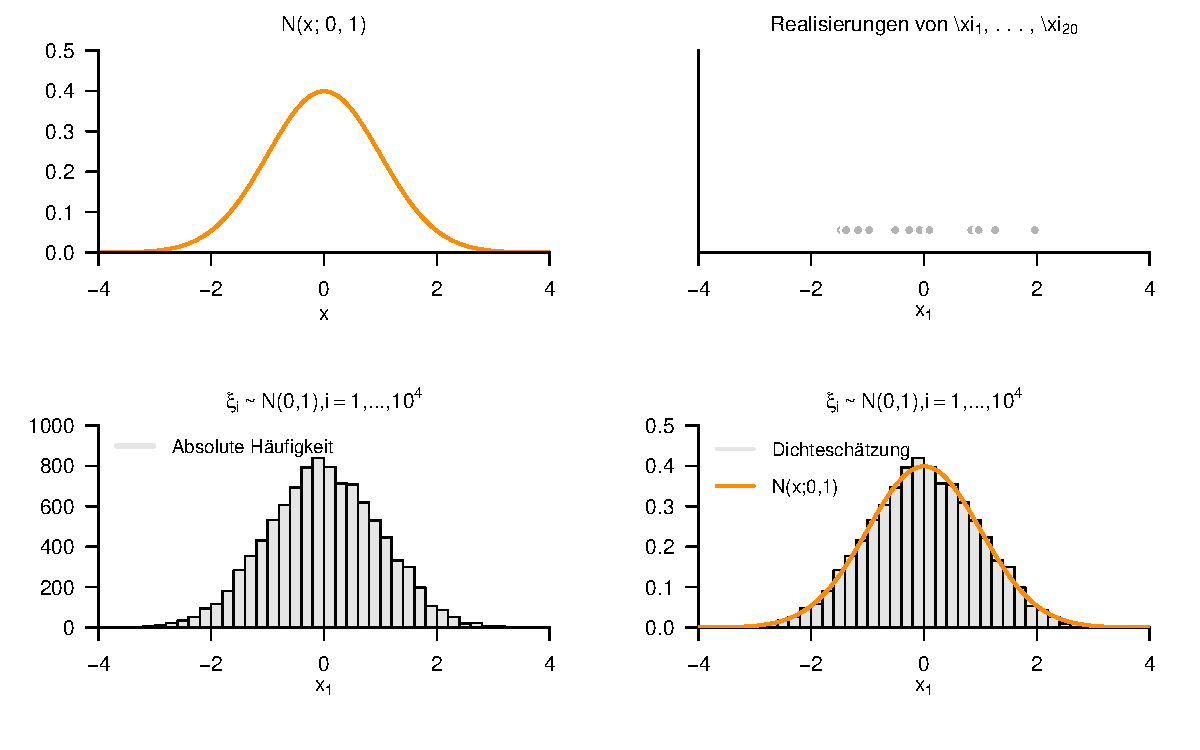
\includegraphics[width=0.9\linewidth]{8_Abbildungen/wtfi_8_realisierungen} \end{center}
\end{frame}

\begin{frame}{Vorbemerkungen}
\protect\hypertarget{vorbemerkungen-2}{}
Transformation von Zufallsvariablen

\footnotesize

Inhalt dieser Vorlesungseinheit sind einige Gesetzmäßigkeiten zur
Transformation von normalverteilten Zufallsvariablen. Mit
\textit{Transformation} ist hier die Anwendung einer Funktion auf
Zufallsvariablen sowie die arithmetische Verknüpfung mehrerer
Zufallsvariablen gemeint. Die zentrale Fragestellung dabei ist folgende:
``Wenn die Zufallsvariable \(\xi\) normalverteilt ist, wie ist dann eine
Zufallsvariable \(\ups\), die sich durch Transformation von \(\xi\)
ergibt, verteilt?''

Für die in dieser Vorlesungseinheit behandelten Fälle gilt, dass man
explizit Wahrscheinlichkeitsdichtefunktionen für die Verteilung der
transformierten Zufallsvariable angeben kann. Diese gehören zu den
klassischen Resultaten der frequentistischen Inferenz und sind für das
Verständnis von Konfidenzintervallen, Hypothesentests, und
Varianzanalysen essentiell.

Intuitiv kann man sich die Transformation einer Zufallsvariable anhand
der Transformation ihrer u.i.v. Realisierungen klar machen. Betrachtet
man z.B. \(\xi \sim N(0,1)\) und ihre Transformation \(\ups := \xi^2\)
und sind \(x_1 = 0.10, x_2 = -0.20, x_3 = 0.80\) drei u.i.v.
Realisierungen von \(\xi\), so entspricht dies den u.i.v. Realisierungen
\(y_1 = x_1^2 = 0.01, y_2 = x_2^2 = 0.04, y_3 = x_3^2 = 0.64\) von
\(\ups\). In diesem Beispiel fällt auf, dass \(\ups\) keine negativen
Werte annimmt, die Verteilung von \(\ups\) ordnet negativen Werten daher
Wahrscheinlichkeitsdichten von \(0\) zu.
\end{frame}

\begin{frame}[fragile]{Vorbemerkungen}
\protect\hypertarget{vorbemerkungen-3}{}
Simulation der Transformation normalverteilter Zufallsvariablen in R

\vspace{2mm}
\footnotesize

\begin{Shaded}
\begin{Highlighting}[]
\CommentTok{\# Simulationsspezifikation}
\NormalTok{n       }\OtherTok{=} \FloatTok{1e4}                          \CommentTok{\# Anzahl von u.i.v Realisierungen (ZVen)}
\NormalTok{mu      }\OtherTok{=} \DecValTok{1}                            \CommentTok{\# Erwartungswertparameter von \textbackslash{}xi}
\NormalTok{sigsqr  }\OtherTok{=} \DecValTok{2}                            \CommentTok{\# Varianzparameter von \textbackslash{}xi}

\CommentTok{\# Quadrieren einer Zufallsvariable}
\NormalTok{x       }\OtherTok{=} \FunctionTok{rnorm}\NormalTok{(n, mu, }\FunctionTok{sqrt}\NormalTok{(sigsqr))   }\CommentTok{\# Realisierungen x\_i, i = 1,....,n von \textbackslash{}xi}
\NormalTok{y       }\OtherTok{=}\NormalTok{ x}\SpecialCharTok{\^{}}\DecValTok{2}                          \CommentTok{\# Realisierungen y\_i = x\_i\^{}2 von \textbackslash{}ups}

\CommentTok{\# Ausgabe der ersten acht Werte}
\FunctionTok{print}\NormalTok{(x[}\DecValTok{1}\SpecialCharTok{:}\DecValTok{8}\NormalTok{], }\AttributeTok{digits =} \DecValTok{2}\NormalTok{)}
\end{Highlighting}
\end{Shaded}

\begin{verbatim}
[1] -1.63  0.26  0.93  1.77 -0.29  1.66  1.51 -0.84
\end{verbatim}

\begin{Shaded}
\begin{Highlighting}[]
\FunctionTok{print}\NormalTok{(y[}\DecValTok{1}\SpecialCharTok{:}\DecValTok{8}\NormalTok{], }\AttributeTok{digits =} \DecValTok{2}\NormalTok{)}
\end{Highlighting}
\end{Shaded}

\begin{verbatim}
[1] 2.672 0.069 0.857 3.126 0.086 2.762 2.290 0.714
\end{verbatim}
\end{frame}

\begin{frame}{Vorbemerkungen}
\protect\hypertarget{vorbemerkungen-4}{}
Simulation der Transformation normalverteilter Zufallsvariablen in R

\vspace{4mm}

\begin{center}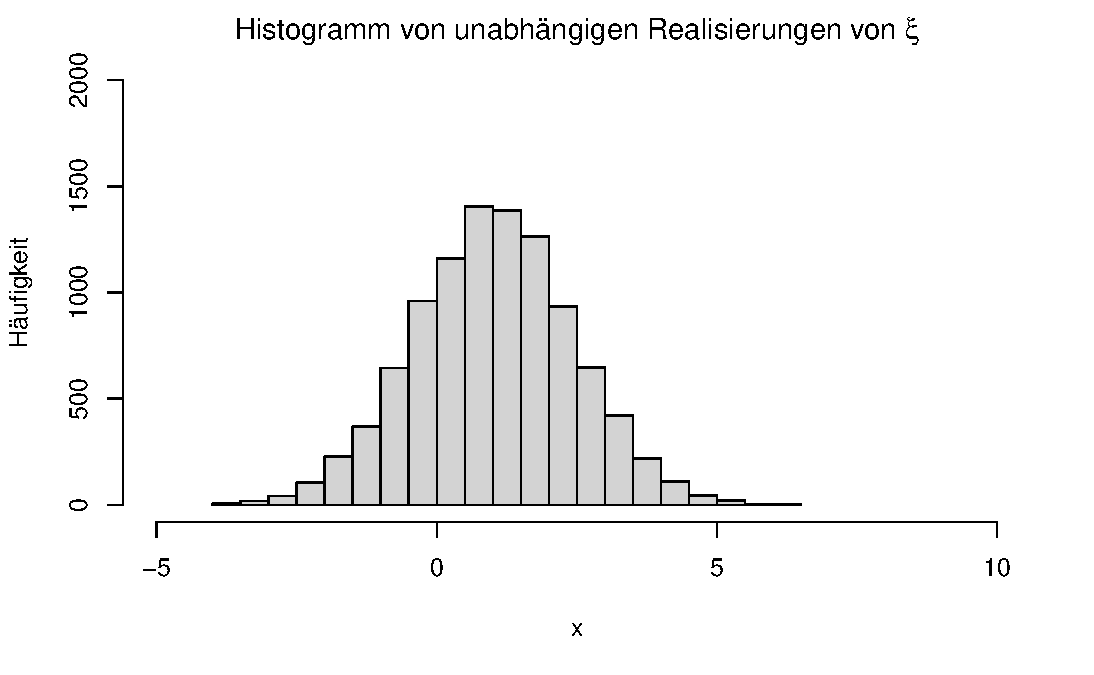
\includegraphics[width=0.9\linewidth]{8_Abbildungen/wtfi_8_hist_x} \end{center}
\end{frame}

\begin{frame}{Vorbemerkungen}
\protect\hypertarget{vorbemerkungen-5}{}
Simulation der Transformation normalverteilter Zufallsvariablen in R

\vspace{4mm}
\center

\begin{center}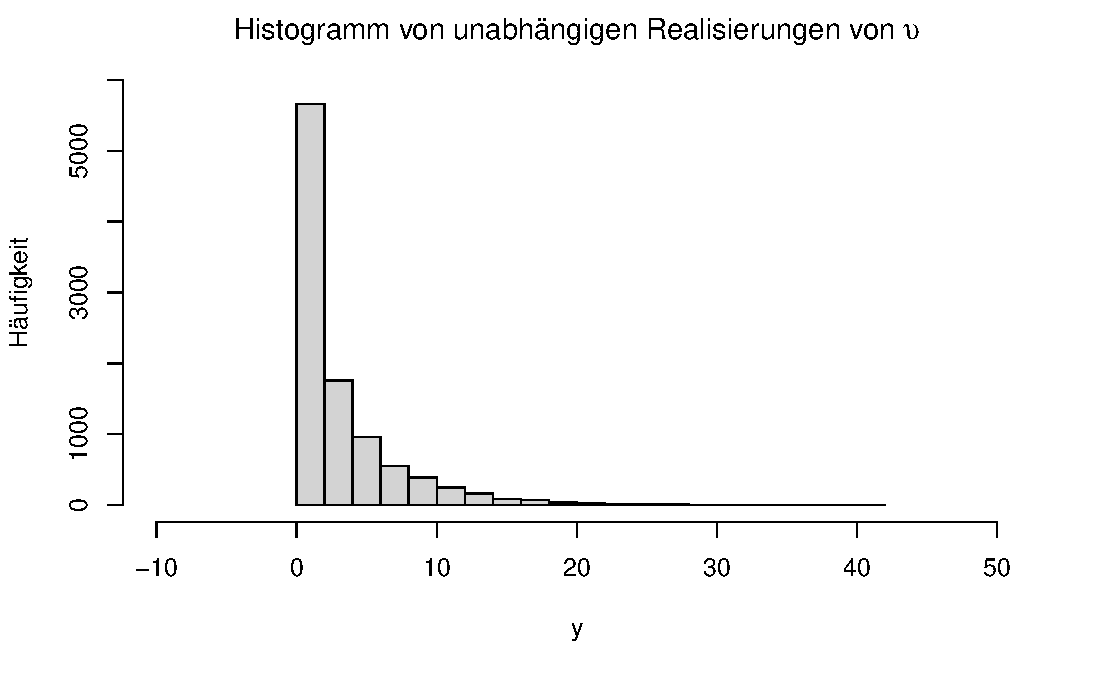
\includegraphics[width=0.9\linewidth]{8_Abbildungen/wtfi_8_hist_y} \end{center}
\end{frame}

\begin{frame}{Vorbemerkungen}
\protect\hypertarget{vorbemerkungen-6}{}
\footnotesize
\begin{theorem}[Transformation eines Zufallsvektors]
\normalfont
\justifying
$\xi : \Omega \to \mathcal{X}$ sei ein Zufallsvektor und $f:\mathcal{X} \to \mathbb{R}^m$ 
sei eine multivariate vektorwertige Funktion. Dann ist
\begin{equation}
\ups : \Omega \to \mathbb{R}, \omega \mapsto \ups(\omega) := (f \circ \xi)(\omega) := f(\xi(\omega))
\end{equation}
ein Zufallsvektor.
\end{theorem}

Bemerkungen

\begin{itemize}
\tightlist
\item
  \justifying Das Theorem formalisiert die oben etablierte Intuition,
  dass die Anwendung einer (deterministischen) Funktion auf eine
  zufällige Größe im Allgemeinen wieder eine zufällige Größe ergibt. Wir
  verzichten auf einen Beweis.
\item
  In einem Beweis müsste die Messbarkeit von \(\ups\) als Folge der
  Messbarkeit von \(\xi\) nachgewiesen werden.
\item
  Im Folgenden ist oft \(\mathcal{X} := \mathbb{R}\) und
  \(f : \mathbb{R} \to \mathbb{R}\).
\item
  Wir schreiben in diesem Fall in der Regel einfach \(\ups := f(\xi)\)
  und nennen \(\ups\) die \emph{transformierte Zufallsvariable}.
\end{itemize}
\end{frame}

\begin{frame}{Vorbemerkungen}
\protect\hypertarget{vorbemerkungen-7}{}
Überblick

\footnotesize
\justifying

Im Abschnitt \textbf{Transformationstheoreme} stellen wir zunächst
einige generelle Werkzeuge zum Berechnen der WDFen von transformierten
Zufallsvariablen bereit. Diese Werkzeuge sind von der allgemeinen Form
``Wenn \(\xi\) eine Zufallsvariable mit WDF \(p_\xi\) und
\(\ups := f(\xi)\) die durch \(f\) transformierte Zufallsvariable ist,
dann gilt für die WDF von \(\ups\) die folgende Formel:
\(p_\ups := \{\mbox{Formel}\}\)''.

Im Abschnitt \textbf{Standardtransformationen} diskutieren wir sechs
Standardtransformationen normalverteilter Zufallsvariablen, die in der
frequentistischen Inferenz und damit im weiteren Verlauf des Kurses
zentrale Rollen spielen. Diese Aussagen sind von der allgemeinen Form
``Wenn \(\xi_i, i = 1,...,n\) unabhängig und identisch normalverteilte
Zufallsvariablen sind und \(\ups := f(\xi_1,...,\xi_n)\) eine
Transformation dieser Zufallsvariablen ist, dann ist die WDF von
\(\ups\) durch die Formel \(p_\ups := \{\mbox{Formel}\}\) gegeben und
man nennt die Verteilung von \(\ups\) \emph{Verteilungsname}''.

Die Aussagen im Abschnitt \textbf{Standardtransformationen} sind für die
frequentistische Inferenz zentral, weil

\begin{enumerate}
[(1)]
\tightlist
\item
  \justifying die Zentralen Grenzwertsätze die Annahme additiv
  unabhängig normalverteilter Störvariablen, und damit normalverteilter
  Daten, rechtfertigt,
\item
  wie wir in der nächsten Vorlesungseinheit sehen werden, es sich bei
  Schätzern und Statistiken um Transformationen von Zufallsvariablen
  handelt, und
\item
  Konfidenzintervalle und Hypothesentests durch die Verteilungen ihrer
  jeweiligen Statistiken charakterisiert und gerechtfertigt sind.
\end{enumerate}
\end{frame}

\begin{frame}{Vorbemerkungen}
\protect\hypertarget{vorbemerkungen-8}{}
Ausblick

\footnotesize

Das probabilistische Standardmodell von \(n\) Datenpunkten hat die Form

\begin{equation}
y_i := \mu_i + \varepsilon_i, i = 1,...,n.
\end{equation}

Die Zufallsvariable \(y_i\) dient dabei als das Modell des \(i\)ten
Datenpunktes \(\tilde{y}_i \in \mathbb{R}\), d.h. \(\tilde{y}_i\) wird
als Realisierung von \(y_i\) modelliert. Die Normalverteilung
\(y_i \sim N(\mu_i,\varepsilon)\) der Zufallsvariable \(y_i\) ergibt
sich dabei wie wir später sehen werden aus der linear-affinen
Transformation der Zufallsvariable \(\varepsilon_i\) unter der Abbildung
\(f(\varepsilon_i) := \mu_i + \varepsilon_i\)

\(\mu_i \in \mathbb{R}\) repräsentiert den deterministischen Aspekt des
Datenpunktmodells und liefert die theoretische Erklärung für den Wert
von \(y_i\). \(\varepsilon_i \sim N(0,\sigma^2)\) dagegen repräsentiert
den stochastischen Aspekt des Datenpunktmodells und liefert im Sinne der
Zentralen Grenzwertsätzte die theoretischer Erklärung für die Differenz
von \(\mu_i\) und \(y_i\) als Resultat der Addition vieler weiterer
Einflüsse in der Generation von \(y_i\) über \(\mu_i\) hinaus.

Statistiken und Schätzer, also Funktionen von \(y_i, i = 1,...,n\),
entsprechen damit im probabilistischen Standardmodell Transformationen
von normalverteilten Zufallsvariablen.
\end{frame}

\begin{frame}{}
\protect\hypertarget{section-4}{}
\setstretch{1.6}
\large

Vorbemerkungen

\textbf{Transformationstheoreme}

Standardtransformationen

\normalsize

\begin{itemize}
\tightlist
\item
  Summentransformation
\item
  Mittelwerttransformation
\item
  \(Z\)-Transformation
\item
  \(\chi^2\)-Transformation
\item
  \(T\)-Transformation
\item
  \(F\)-Transformation
\end{itemize}

\large

Selbstkontrollfragen
\end{frame}

\begin{frame}{Transformationstheoreme}
\protect\hypertarget{transformationstheoreme}{}
Überblick

\footnotesize
\justifying

Das \textbf{univariate WDF Transformationstheorem bei bijektiven
Abbildungen} liefert eine Formel zur Berechnung der WDF \(p_\ups\) von
\(\ups := f(\xi)\), wenn \(\xi\) eine Zufallsvariable mit WDF \(p_\xi\)
ist und \(f\) eine bijektive Funktion ist.

Das \textbf{univariate WDF Transformationstheorem bei linear affinen
Abbildungen} gibt eine Formel zur Berechnung der WDF \(p_\ups\) von
\(\ups := f(\xi)\) an, wenn \(\xi\) eine Zufallsvariable mit WDF
\(p_\xi\) ist und \(f\) eine linear-affine Funktion ist.

Das \textbf{univariate WDF Transformationstheorem bei stückweisen
bijektiven Abbildungen} gibt eine Formel zur Berechnung der WDF
\(p_\ups\) von \(\ups := f(\xi)\) an, wenn \(\xi\) eine Zufallsvariable
mit WDF \(p_\xi\) ist und \(f\) zumindest in Teilen bijektiv ist.

Das \textbf{multivariate WDF Transformationstheorem bei bijektiven
Abbildungen} liefert eine Formel zur Berechnung der WDF \(p_\ups\) von
\(\ups := f(\xi)\), wenn \(\xi\) ein Zufallsvektor mit WDF \(p_\xi\) ist
und \(f\) eine bijektive multivariate vektorwertigeFunktion ist.

Das \textbf{Faltungstheorem} liefert eine Formel zur Berechnung der WDF
\(p_\ups\) von \(\ups := \xi_1 + \xi_2\), wenn \(\xi_1\) und \(\xi_2\)
zwei Zufallsvariablen mit WDFen \(p_{\xi_1}\) und \(p_{\xi_2}\) sind.
\end{frame}

\begin{frame}{Transformationstheoreme}
\protect\hypertarget{transformationstheoreme-1}{}
\small
\begin{theorem}[Univariate WDF Transformation bei bijektiven Abbildungen]
\normalfont
\justifying
$\xi$ sei eine Zufallsvariable mit WDF $p_\xi$ für die $\mathbb{P}(]a,b[) = 1$ gilt,
wobei $a$ und/oder $b$ entweder endlich oder unendlich seien. Weiterhin sei
\begin{equation}
\ups := f(\xi)
\end{equation}
wobei die univariate reellwertige Funktion $f : ]a,b[ \to \mathbb{R}$ differenzierbar
und bijektiv auf $]a,b[$ sei. $f(]a,b[)$ sei das Bild von $]a,b[$ unter $f$.
Schließlich sei $f^{-1}(y)$ der Wert der Umkehrunktion von $f(x)$ für
$y \in f(]a,b[)$ und $f'(x)$ sei die Ableitung von $f$ an der Stelle $x$.
Dann ist die WDF von $\ups$ gegeben durch
\begin{equation}
p_\ups : \mathbb{R} \to \mathbb{R}_{\ge 0}, y \mapsto p_\ups(y) :=
\begin{cases}
\frac{1}{\vert  f^{'}\left(f^{-1}(y)\right) \vert}p_\xi\left(f^{-1}(y)\right)
& \mbox{ für } y \in f(]a,b[) \\
0
& \mbox{ für } y \in \mathbb{R} \setminus f(]a,b[).
\end{cases}
\end{equation}
\end{theorem}

\footnotesize

Bemerkungen

\begin{itemize}
\tightlist
\item
  Linear-affine Abbildungen sind ein wichtiger Anwendungsfalls.
\item
  Die \(Z\)-Transformation ist ein wichtiger Anwendungsfall.
\end{itemize}
\end{frame}

\begin{frame}{Transformationstheoreme}
\protect\hypertarget{transformationstheoreme-2}{}
\tiny
\setstretch{1}

\underline{Beweis}

Wir halten zunächst fest, dass weil \(f\) eine differenzierbare
bijektive Funktion auf \(]a,b[\) ist, \(f\) entweder strikt wachsend
oder strikt fallend ist. Nehmen wir zunächst an, dass \(f\) auf
\(]a,b[\) strikt wachsend ist. Dann ist auch \(f^{-1}\) für alle
\(y \in f(]a,b[)\) wachsend, und es gilt \begin{equation*}
P_\ups(y)
= \mathbb{P}(\ups \le y)
= \mathbb{P}\left(f(\xi) \le y\right)
= \mathbb{P}\left(f^{-1}(f(\xi)) \le f^{-1}(y)\right)
= \mathbb{P}\left(\xi \le f^{-1}(y)\right)
= P_\xi\left(f^{-1}(y)\right).
\end{equation*} \(P_\ups\) ist also differenzierbar an allen Stellen
\(y\), an denen sowohl \(f^{-1}\) als auch \(P_\xi\) differenzierbar
sind. Mit der Kettenregel und dem Satz von der Umkehrabbildung
\((f^{-1}(x))' = 1/f'(f^{-1}(x))\), folgt dann, dass die WDF \(p_\ups\)
sich ergibt wie folgt: \begin{equation*}
p_\ups(y)
= \frac{d}{dy}P_\ups(y)
= \frac{d}{dy}P_\xi\left(f^{-1}(y)\right)
= p_\xi\left(f^{-1}(y)\right)\frac{d}{dy}f^{-1}(y)
= \frac{1}{f'\left(f^{-1}(y)\right)} p_\xi\left(f^{-1}(y)\right),
\end{equation*} Weil \(f^{-1}\) strikt wachsend ist, ist
\(d/dy (f^{-1}(y))\) positiv und das Theorem trifft zu. Analog gilt,
dass wenn \(f\) auf \(]a,b[\) strikt fallend ist, dann ist auch
\(f^{-1}\) für alle \(y \in f(]a,b[)\) fallend und es gilt
\begin{equation*}
P_\ups(y)
= \mathbb{P}(f(\xi) \le y)
= \mathbb{P}\left(f^{-1}(f(\xi)) \ge f^{-1}(y)\right)
= \mathbb{P}\left(\xi \ge f^{-1}(y)\right)
= 1 - P_\xi\left(f^{-1}(y) \right),
\end{equation*} Mit der Kettenregel und dem Satz von der Umkehrabbildung
folgt dann \begin{equation*}
p_\ups(y)
= \frac{d}{dy}(1 - P_\ups(y))
= -\frac{d}{dy}P_\xi\left(f^{-1}(y)\right)
= -p_\xi\left(f^{-1}(y)\right)\frac{d}{dy}f^{-1}(y)
= -\frac{1}{f'\left(f^{-1}(y)\right)} p_\xi\left(f^{-1}(y)\right).
\end{equation*} Weil \(f^{-1}\) strikt fallend ist, ist
\(d/dy (f^{-1}(y))\) negativ, so dass \(-d/dy (f^{-1}(y))\) gleich
\(|d/dy (f^{-1}(y))|\) ist und das Theorem trifft zu.
\end{frame}

\begin{frame}{Transformationstheoreme}
\protect\hypertarget{transformationstheoreme-3}{}
\small
\begin{theorem}[Univariate WDF Transformation bei linear-affinen Abbildungen]
\normalfont
\justifying
$\xi$ sei eine Zufallsvariable mit WDF $p_\xi$ und es sei
\begin{equation}
\ups = f(\xi) \mbox{ mit } f(\xi) := a\xi + b \mbox{ für } a\neq 0.
\end{equation}
Dann ist die WDF von $\ups$ gegeben durch
\begin{equation}
p_\ups : \mathbb{R} \to \mathbb{R}_{\ge 0}, y \mapsto p_\ups(y) :=
\frac{1}{|a|}p_\xi\left(\frac{y-b}{a}\right).
\end{equation}
\end{theorem}

Bemerkung

\begin{itemize}
\tightlist
\item
  Das Theorem folgt direkt WDF Transformationstheorem bei bijektiven
  Abbildungen.
\item
  Die \(Z\)-Transformation ist ein wichtiger Anwendungsfall.
\end{itemize}
\end{frame}

\begin{frame}{Transformationstheoreme}
\protect\hypertarget{transformationstheoreme-4}{}
\footnotesize

\underline{Beweis} \vspace{1mm}

Wir halten zunächst fest, dass \begin{equation}
f^{-1} : \mathbb{R} \to \mathbb{R}, y  \mapsto f^{-1}(y) = \frac{y - b}{a}
\end{equation} ist, weil dann
\(f \circ f^{-1} = \mbox{id}_{\mathbb{R}}\) gilt, wie man anhand von
\begin{equation}
f(f^{-1}(x)) = a \left(\frac{x - b}{a}\right) + b = x - b + b = x \mbox{ für alle } x \in \mathbb{R}
\end{equation} einsieht. Wir halten weiterhin fest, dass
\begin{equation}
f' : \mathbb{R} \to \mathbb{R}, x \mapsto f'(x) = \frac{d}{dx}(ax  + b) = a.
\end{equation} Also folgt mit dem Theorem zur WDF Transformation bei
bijektiven Abbildungen, dass \begin{align}
\begin{split}
p_\ups : \mathbb{R} \to \mathbb{R}_{\ge 0}, y \mapsto p_\ups(y)
& = \frac{1}{\vert f^{'}\left(f^{-1}(y)\right)\vert}p_\xi\left(f^{-1}(y)\right) \\
& = \frac{1}{|a|}p_\xi\left(\frac{y - b}{a}\right).
\end{split}
\end{align} \(\hfill \Box\)
\end{frame}

\begin{frame}{Transformationstheoreme}
\protect\hypertarget{transformationstheoreme-5}{}
\footnotesize
\begin{theorem}[WDF Transformation bei stückweise bijektiven Abbildungen]
\normalfont
\justifying
$\xi$ sei eine Zufallsvariable mit Ergebnisraum $\mathcal{X}$ und WDF $p_\xi$. Weiterhin sei
\begin{equation}
\ups = f(\xi),
\end{equation}
wobei $f$ so beschaffen sei, dass der Ergebnisraum von $\xi$ in eine endliche Anzahl
von Mengen $\mathcal{X}_1,...,\mathcal{X}_k$ mit einer entsprechenden Anzahl von
Mengen $\mathcal{Y}_1 := f(\mathcal{X}_1), ..., \mathcal{Y}_k :=  f(\mathcal{X}_k)$
im Ergebnisraum $\mathcal{Y}$ von $\ups$ partitioniert werden kann (wobei nicht
notwendigerweise $\mathcal{Y}_i \cap \mathcal{Y}_j = \emptyset, 1 \le i,j \le k$
gelten muss), so dass die Abbildung $f$ für alle $\mathcal{X}_1,...,\mathcal{X}_k$
bijektiv ist (d.h. $f$ ist eine \textit{stückweise} bijektive Abbildung). Für
$i = 1,...,k$ bezeichne $f_i^{-1}$ die Umkehrfunktion von $f$ auf $\mathcal{Y}_i$.
Schließlich nehmen wir an, dass die Ableitungen $f_i^{\prime}$ für alle $i=1,...,k$
existieren und stetig sind. Dann ist eine WDF von $\ups$ durch
\begin{equation}
p_\ups : \mathcal{Y} \to \mathbb{R}_{\ge 0}, y \mapsto p_\ups(y) :=
\sum_{i=1}^k 1_{\mathcal{Y}_i} (y) \frac{1}{\vert  f^{'}_i(f^{-1}_i(y)) \vert}p_\xi\left(f^{-1}_i(y)\right).
\end{equation}
gegeben.
\end{theorem}

Bemerkungen

\begin{itemize}
\tightlist
\item
  Wir verzichten auf einen Beweis.
\item
  Die \(\chi^2\)-Transformation ist ein wichtiger Anwendungsfall.
\end{itemize}
\end{frame}

\begin{frame}{Transformationstheoreme}
\protect\hypertarget{transformationstheoreme-6}{}
\footnotesize
\begin{theorem}[Multivariate WDF Transformation bei bijektiven Abbildungen]
\normalfont
\justifying
$\xi$ sei ein $n$-dimensionaler Zufallsvektor mit Ergebnisraum $\mathbb{R}^n$ und
WDF $p_\xi$. Weiterhin sei
\begin{equation}
\ups := f(\xi),
\end{equation}
wobei die multivariate vektorwertige Funktion $f : \mathbb{R}^n \to \mathbb{R}^n$
differenzierbar und bijektiv auf $]a,b[$ sei. Schließlich seien
\begin{equation}
J^f(x)
= \left(\frac{\partial}{\partial x_j}f_i(x)\right)_{1\le i \le n, 1 \le j \le n}
\in \mathbb{R}^{n \times n}
\end{equation}
die Jacobi-Matrix von $f$ an der Stelle $x \in \mathbb{R}^n$, $|J^f(x)|$ die
Determinante von $J^f(x)$, und es sei $|J^f(x)| \neq 0$ für alle $x \in \mathbb{R}^n$.
Dann ist eine WDF von $\ups$ durch
\begin{equation}\label{eq:mpdf_transform}
p_\ups : \mathbb{R}^n \to \mathbb{R}_{\ge 0}, y \mapsto p_\ups(y) :=
\begin{cases}
\frac{1}{|J^f\left(f^{-1}(y)\right)|}p_\xi\left(f^{-1}(y)\right)
& \mbox{ for } y\in f(\mathbb{R}^n) \\
0
& \mbox{ for } y \in \mathbb{R}^n \setminus f(\mathbb{R}^n)
\end{cases}
\end{equation}
gegeben.
\end{theorem}

Bemerkungen

\begin{itemize}
\tightlist
\item
  Wir verzichten auf einen Beweis.
\item
  Es handelt sich um eine direkte Generalisierung des univariaten Falls.
\item
  Die \(T\)-und \(F\)-Transformationen sind wichtige Anwendungsfälle.
\end{itemize}
\end{frame}

\begin{frame}{Transformationstheoreme}
\protect\hypertarget{transformationstheoreme-7}{}
\small
\begin{theorem}[Summe unabhängiger Zufallsvariable, Faltung]
\justifying
\normalfont
$\xi_1$ und $\xi_2$ seien zwei kontinuierliche unabhängige Zufallsvariablen mit WDF
$p_{\xi_1}$ und $p_{\xi_2}$, respektive. $\ups := \xi_1 + \xi_2$ sei die Summe von $\xi_1$
und $\xi_2$. Dann ergibt sich eine WDF der Verteilung von $\ups$ als
\begin{equation}
p_\ups(y)
= \int_{-\infty}^\infty p_{\xi_1}(y - x_2)p_{\xi_2}(x_2)\,dx_2
= \int_{-\infty}^\infty p_{\xi_1}(x_1)p_{\xi_2}(y - x_1)\,dx_1
\end{equation}
Die Formel für die WDF $p_\ups$ heißt \textit{Faltung} oder \textit{Konvolution}
von $p_{\xi_1}$ und $p_{\xi_2}$.
\end{theorem}

\footnotesize

Bemerkung

\begin{itemize}
\tightlist
\item
  Die Summen- und Mittelwerttransformation sind wichtige
  Anwendungsfälle.
\end{itemize}
\end{frame}

\begin{frame}{Transformationstheoreme}
\protect\hypertarget{transformationstheoreme-8}{}
\setstretch{1.1}
\footnotesize

\underline{Beweis} \vspace{2mm}

Wir nutzen das multivariate WDF Transformationstheorem für bijektive
Abbildungen. Dazu definieren wir zunächst \begin{equation}
f : \mathbb{R}^2 \to \mathbb{R}^2, x \mapsto f(x) :=
\begin{pmatrix}
x_1 + x_2 \\
x_2
\end{pmatrix}
:=
\begin{pmatrix}
z_1 \\ z_2
\end{pmatrix}
\end{equation} Die inverse Funktion von \(f\) ist dann gegeben durch
\begin{equation}
f : \mathbb{R}^2 \to \mathbb{R}^2, z \mapsto f(z) :=
\begin{pmatrix}
z_1 - x_2 \\
z_2
\end{pmatrix}
\end{equation} weil dann \(f \circ f^{-1} = \mbox{id}_{\mathbb{R}^2}\)
gilt, wie man anhand von \begin{equation}
f^{-1}\left(f(x)\right)
=
f^{-1}
\begin{pmatrix}
x_1 + x_2 \\
x_2
\end{pmatrix}
=
\begin{pmatrix}
x_1 + x_2 - x_2\\
x_2
\end{pmatrix}
=
\begin{pmatrix}
x_1 \\
x_2
\end{pmatrix}
\end{equation} einsieht. Die Jacobimatrix von \(f\) ergibt sich zu
\begin{equation}
J^{f}(x) =
\begin{pmatrix}
\frac{\partial}{\partial x_1} f_1(x) &  \frac{\partial}{\partial x_2} f_1(x) \\
\frac{\partial}{\partial x_1} f_2(x) &  \frac{\partial}{\partial x_2} f_2(x) \\
\end{pmatrix}
=
\begin{pmatrix}
    \frac{\partial}{\partial x_1} (x_1 + x_2)
&   \frac{\partial}{\partial x_2} (x_1 + x_2)
\\
    \frac{\partial}{\partial x_1} x_2
&   \frac{\partial}{\partial x_2} x_2 \\
\end{pmatrix}
=
\begin{pmatrix}
1 &  1 \\
0 &  1 \\
\end{pmatrix}
\end{equation} und die Jacobideterminante damit zu \(|J^f(x)| = 1\).
\end{frame}

\begin{frame}{Transformationstheoreme}
\protect\hypertarget{transformationstheoreme-9}{}
\setstretch{1.1}
\footnotesize

\underline{Beweis (fortgeführt)} \vspace{2mm}

Wir halten weiterhin fest, dass die Unabhängigkeit von \(\xi_1\) und
\(\xi_2\) impliziert, dass \begin{equation}
p_{\xi_1,\xi_2}(x_1,x_2) = p_{\xi_1}(x_1)p_{\xi_2}(x_2)
\end{equation} impliziert. Einsetzen und Integration hinsichtlich
\(x_2\) ergibt dann ergibt dann für \(z \in f(\mathbb{R}^2)\)
\begin{align}
\begin{split}
p_\zeta(z)
& = \frac{1}{|J^f\left(f^{-1}(z)\right)|}p_\xi\left(f^{-1}(z)\right)  \\
& = \frac{1}{1}p_{\xi_1,\xi_2}\left(z_1 - x_2, x_2\right)  \\
& = p_{\xi_1}(z_1 - x_2)p_{\xi_2}(x_2)
\end{split}
\end{align} Integration über \(x_2\) ergibt dann eine WDF für die
marginale Verteilung von \(\zeta_1\) \begin{align}
\begin{split}
p_{\zeta_1}(z_1)
& = \int_{-\infty}^{\infty} p_{\xi_1}(z_1 - x_2)p_{\xi_2}(x_2)\,dx_2
\end{split}
\end{align} Mit \(\zeta_1 = \xi_1 + \xi_2 = \ups\) ergibt sich dann die
erste Form des Faltungstheorems zu \begin{align}
p_\ups(y)
& = \int_{-\infty}^{\infty} p_{\xi_1}(y - x_2)p_{\xi_2}(x_2)\,dx_2.
\end{align} \(\hfill \Box\)
\end{frame}

\begin{frame}{}
\protect\hypertarget{section-5}{}
\setstretch{1.6}
\large

Vorbemerkungen

Transformationstheoreme

\textbf{Standardtransformationen}

\normalsize

\begin{itemize}
\tightlist
\item
  Summentransformation
\item
  Mittelwerttransformation
\item
  \(Z\)-Transformation
\item
  \(\chi^2\)-Transformation
\item
  \(T\)-Transformation
\item
  \(F\)-Transformation
\end{itemize}

\large

Selbstkontrollfragen
\end{frame}

\begin{frame}{Standardtransformationen}
\protect\hypertarget{standardtransformationen}{}
Überblick \vspace{1mm}

\justifying
\footnotesize

Das \textbf{Summentransformationstheorem} besagt, dass die Summe
unabhängig normalverteilter Zufallsvariablen wiederum normalverteilt ist
und gibt die Parameter dieser Verteilung an.

Das \textbf{Mittelwertstransformationstheorem} besagt, dass das
Stichprobenmittel unabhängig normalverteilter Zufallsvariablen wiederum
normalverteilt ist und gibt die Parameter dieser Verteilung an.

Das \textbf{\(Z\)-Transformationstheorem} besagt, dass Subtraktion des
Erwartungswertparameters und gleichzeitige Division mit der Wurzel des
Varianzsparameters die Verteilung einer normalverteilten Zufallsvariable
in eine Standardnormalverteilung transformiert.

Das \textbf{\(\chi^2\)-Transformationstheorem} besagt, dass die Summe
quadrierter unabhängiger standardnormalverteilter Zufallsvariablen eine
\(\chi^2\)-verteilte Zufallsvariable ist.

Das \textbf{\(T\)-Transformationstheorem} besagt, dass die
Zufallsvariable, die sich durch Division einer standardnormalverteilten
Zufallsvariable durch die Quadratwurzel einer \(\chi^2\)-verteilten
Zufallsvariable geteilt durch ein \(n\), ergibt, eine \(t\)-verteilte
Zufallsvariable ist.

Das \textbf{\(F\)-Transformationstheorem} besagt, dass die
Zufallsvariable, die sich durch Division zweier \(\chi^2\) verteilter
Zufallsvariablen, jeweils geteilt durch ihre jeweiligen
Freiheitsgradparameter, ergibt eine \(F\)-verteilte Zufallsvariable ist.
\end{frame}

\begin{frame}{}
\protect\hypertarget{section-6}{}
\setstretch{1.6}
\large

Vorbemerkungen

Transformationstheoreme

\textbf{Standardtransformationen}

\normalsize

\begin{itemize}
\tightlist
\item
  \textbf{Summentransformation}
\item
  Mittelwerttransformation
\item
  \(Z\)-Transformation
\item
  \(\chi^2\)-Transformation
\item
  \(T\)-Transformation
\item
  \(F\)-Transformation
\end{itemize}

\large

Selbstkontrollfragen
\end{frame}

\begin{frame}{Summentransformation}
\protect\hypertarget{summentransformation}{}
\small
\begin{theorem}[Summe unabhängig normalverteilter Zufallsvariablen]
\justifying
\normalfont
Für $i = 1,...,n$ seien $\xi_i \sim N(\mu_i,\sigma^2_i)$ unabhängige normalverteilte
Zufallsvariablen. Dann gilt für die Summe $\ups := \sum_{i=1}^n \xi_i$ , dass
\begin{equation}
\ups \sim N\left(\sum_{i=1}^n \mu_i, \sum_{i=1}^n \sigma^2_i\right)
\end{equation}
Für unabhängige und identisch normalverteilte Zufallsvariablen
$\xi_i \sim N(\mu,\sigma^2)$ gilt folglich
\begin{equation}
\ups \sim N(n\mu, n \sigma^2).
\end{equation}
\end{theorem}

\footnotesize

Bemerkungen

\begin{itemize}
\tightlist
\item
  Die Mittelwerttransformation ist ein wichtiger Anwendungsfall.
\item
  Die Generalisierung der zentralen Grenzwertsätze sind wichtige
  Anwendungsfälle.
\end{itemize}
\end{frame}

\begin{frame}{Summentransformation}
\protect\hypertarget{summentransformation-1}{}
\vfill

\begin{center}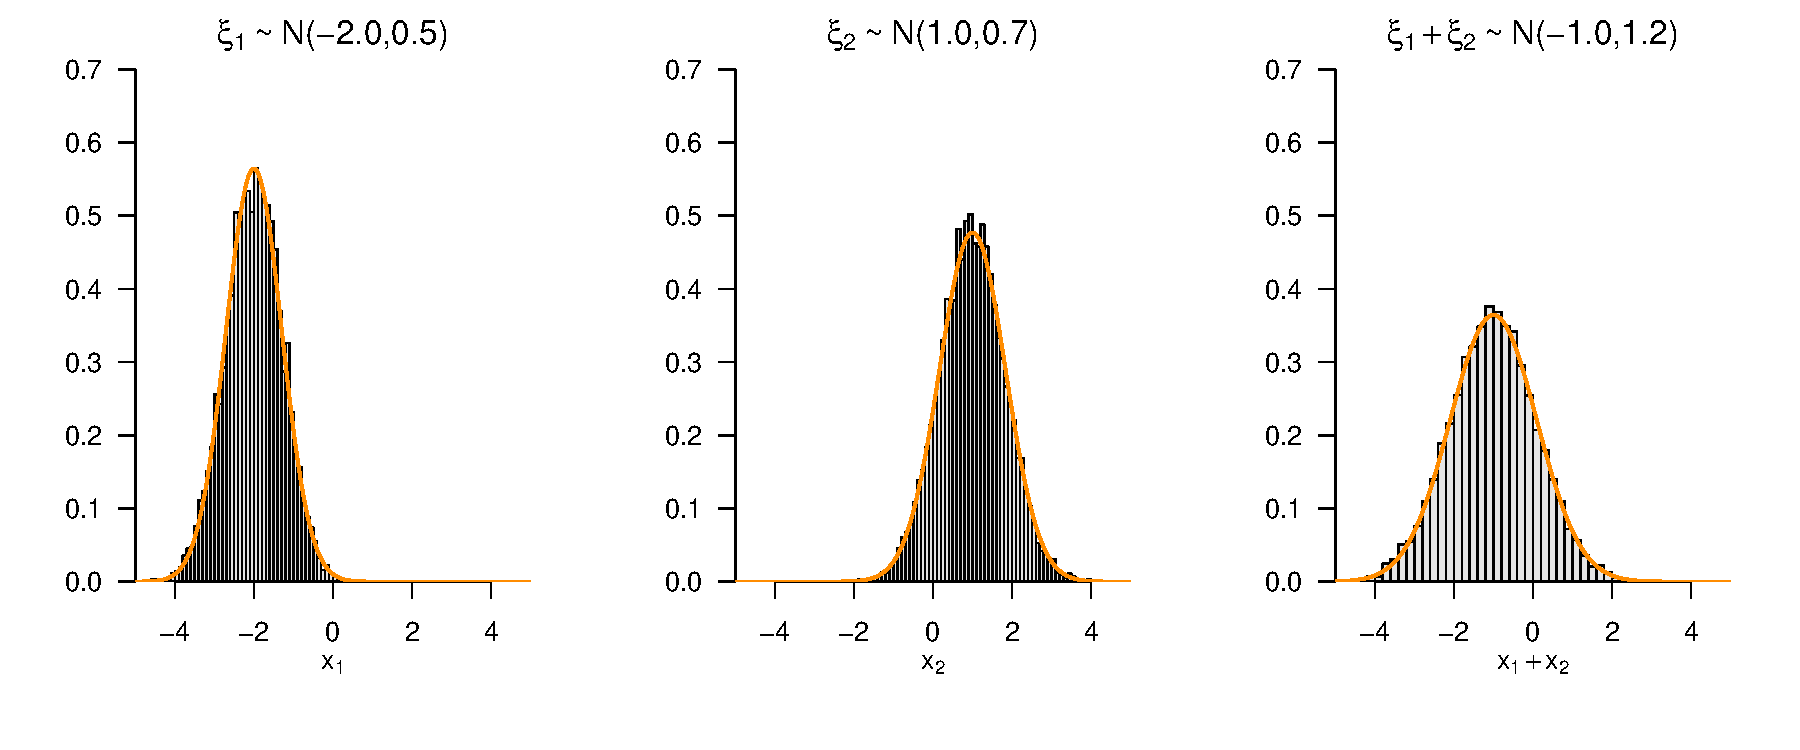
\includegraphics[width=1\linewidth]{8_Abbildungen/wtfi_8_summation} \end{center}
\vfill
\end{frame}

\begin{frame}{Summentransformation}
\protect\hypertarget{summentransformation-2}{}
\footnotesize

\underline{Beweis}

Wir skizzieren mithilfe der Faltungsformel, dass für
\(\xi_1 \sim N(\mu_1,\sigma^2_1)\), \(\xi_2 \sim N(\mu_2,\sigma^2_2)\),
und \(\ups := \xi_1 + \xi_2\) gilt, dass
\(\ups \sim N(\mu_1 + \mu_2,\sigma_1^2 + \sigma_2^2)\). Für \(n > 2\)
folgt das Theorem dann durch Iteration. Mit der Definition der WDF der
Normalverteilung erhalten wir zunächst \begin{align}
\begin{split}
p_\ups(y)
& = \int_{-\infty}^\infty p_{\xi_1}(x_1)p_{\xi_2}(y - x_1)\,dx_1
\\
& = \int_{-\infty}^\infty
    \frac{1}{\sqrt{2 \pi} \sigma_1} \exp\left(-\frac{1}{2}\left(\frac{x_1 - \mu_1}{\sigma_1}\right)^2\right)
    \frac{1}{\sqrt{2 \pi} \sigma_2} \exp\left(-\frac{1}{2}\left(\frac{y - x_1 - \mu_2}{\sigma_2}\right)^2\right)
    \,dx_1
\\
& = \int_{-\infty}^\infty
    \frac{1}{2 \pi \sigma_1\sigma_2}\exp
    \left(
    -\frac{1}{2}\left(\frac{x_1 - \mu_1}{\sigma_1}\right)^2
    -\frac{1}{2}\left(\frac{y - x_1 - \mu_2}{\sigma_2}\right)^2
    \right)
    \,dx_1 .
\\
\end{split}
\end{align} Mit einigem algebraischen Aufwand erhält man die Identität
\begin{multline}
-\frac{1}{2}\left(\frac{x_1 - \mu_1}{\sigma_1}\right)^2
-\frac{1}{2}\left(\frac{y - x_1 - \mu_2}{\sigma_2}\right)^2
\\ =
-\frac{(y - \mu_1 - \mu_2)^2}
      {2(\sigma_1^2 + \sigma_2^2)}
-\frac{((\sigma_1^2 + \sigma_2^2)x_1 -\sigma_1^2y + \mu_2 \sigma_1^2 - \mu_1 \sigma_2^2)^2}
      {2\sigma_1^2\sigma_2^2(\sigma_1^2 + \sigma_2^2)},
\end{multline} so dass weiterhin gilt, dass
\end{frame}

\begin{frame}{Summentransformation}
\protect\hypertarget{summentransformation-3}{}
\footnotesize

\underline{Beweis (fortgeführt)}

\tiny

\begin{align}
\begin{split}
p_\ups(y)
& = \int_{-\infty}^\infty
    \frac{1}{2 \pi \sigma_1\sigma_2}
    \exp\left(
    -\frac{(y - \mu_1 - \mu_2)^2}
      {2(\sigma_1^2 + \sigma_2^2)}
    -\frac{((\sigma_1^2 + \sigma_2^2)x_1 -\sigma_1^2y + \mu_2 \sigma_1^2 - \mu_1 \sigma_2^2)^2}
      {2\sigma_1^2\sigma_2^2(\sigma_1^2 + \sigma_2^2)}
    \right)
    \,dx_1
\\
& = \int_{-\infty}^\infty
    \frac{1}{2 \pi \sigma_1\sigma_2}
    \exp\left(
    -\frac{(y - \mu_1 - \mu_2)^2}
      {2(\sigma_1^2 + \sigma_2^2)}
    \right)
    \exp\left(
    -\frac{((\sigma_1^2 + \sigma_2^2)x_1 -\sigma_1^2y + \mu_2 \sigma_1^2 - \mu_1 \sigma_2^2)^2}
      {2\sigma_1^2\sigma_2^2(\sigma_1^2 + \sigma_2^2)}
    \right)
    \,dx_1
\\
& = \frac{1}{2 \pi \sigma_1\sigma_2}
    \exp\left(
    -\frac{(y - \mu_1 - \mu_2)^2}
      {2(\sigma_1^2 + \sigma_2^2)}
    \right)
    \int_{-\infty}^\infty
    \exp\left(
    -\frac{((\sigma_1^2 + \sigma_2^2)x_1 -\sigma_1^2y + \mu_2 \sigma_1^2 - \mu_1 \sigma_2^2)^2}
      {2\sigma_1^2\sigma_2^2(\sigma_1^2 + \sigma_2^2)}
    \right)
    \,dx_1.
\end{split}
\end{align}
\end{frame}

\begin{frame}{Summentransformation}
\protect\hypertarget{summentransformation-4}{}
\footnotesize

\underline{Beweis (fortgeführt)}

Für das verbleibende Integral zeigt man mithilfe der Integration durch
Substitution, dass \begin{equation}
\int_{-\infty}^\infty
    \exp\left(
    -\frac{((\sigma_1^2 + \sigma_2^2)x_1 -\sigma_1^2y + \mu_2 \sigma_1^2 - \mu_1 \sigma_2^2)^2}
      {2\sigma_1^2\sigma_2^2(\sigma_1^2 + \sigma_2^2)}
    \right)
    \,dx_1
= \frac{\sqrt{2\pi}\sigma_1\sigma_2}{\sqrt{\sigma_1^2 + \sigma_2^2}}.
\end{equation} Es ergibt sich also \begin{align}
\begin{split}
p_\ups(y)
& = \frac{1}{2 \pi \sigma_1\sigma_2}
    \frac{\sqrt{2\pi}\sigma_1\sigma_2}{\sqrt{\sigma_1^2 + \sigma_2^2}}
    \exp\left(
    -\frac{(y - \mu_1 - \mu_2)^2}
      {2(\sigma_1^2 + \sigma_2^2)}
    \right)
\\
& = \frac{(2\pi)^{-1}(2\pi)^2}{\sqrt{\sigma_1^2 + \sigma_2^2}}
    \exp\left(
    -\frac{(y - \mu_1 - \mu_2)^2}
      {2(\sigma_1^2 + \sigma_2^2)}
    \right)
\\
& = \frac{1}{\sqrt{2\pi}\sqrt{\sigma_1^2 + \sigma_2^2}}
    \exp\left(
    -\frac{(y - \mu_1 - \mu_2)^2}
      {2(\sigma_1^2 + \sigma_2^2)}
    \right).
\end{split}
\end{align}
\end{frame}

\begin{frame}{Summentransformation}
\protect\hypertarget{summentransformation-5}{}
\footnotesize

\underline{Beweis (fortgeführt)} \vspace{2mm}

Schließlich folgt, dass \begin{align}
\begin{split}
p_\ups(y)
& = \frac{1}{\sqrt{2\pi(\sigma_1^2 + \sigma_2^2)}}
  \exp\left(-\frac{1}{2(\sigma_1^2 + \sigma_2^2)}\left(y - (\mu_1 + \mu_2)\right)^2\right) \\
& = N(y; \mu_1 + \mu_2, \sigma_1^2 + \sigma_2^2)
\end{split}
\end{align} Ein einfacheres Vorgehen ergibt sich vermutlich nach
Fouriertransformation der WDF im Sinne der sogenannten
charakteristischen Funktion einer Zufallsvariable. In diesem Fall würde
die Faltung der WDFen der Multiplikation der charakteristischen
Funktionen entsprechen.

\(\hfill \Box\)
\end{frame}

\begin{frame}{}
\protect\hypertarget{section-7}{}
\setstretch{1.6}
\large

Vorbemerkungen

Transformationstheoreme

\textbf{Standardtransformationen}

\normalsize

\begin{itemize}
\tightlist
\item
  Summentransformation
\item
  \textbf{Mittelwerttransformation}
\item
  \(Z\)-Transformation
\item
  \(\chi^2\)-Transformation
\item
  \(T\)-Transformation
\item
  \(F\)-Transformation
\end{itemize}

\large

Selbstkontrollfragen
\end{frame}

\begin{frame}{Mittelwerttransformation}
\protect\hypertarget{mittelwerttransformation}{}
\small
\begin{theorem}[Stichprobenmittel von u.i.v. normalverteilten Zufallsvariablen]
\justifying
\normalfont
Für $i = 1,...,n$ seien $\xi_i \sim N(\mu,\sigma^2)$ unabhängig und identisch
normalverteilte Zufallsvariablen. Dann gilt für das Stichprobenmittel
$\bar{\xi}_n := \frac{1}{n}\sum_{i=1}^n \xi_i$ , dass
\begin{equation}
\bar{\xi}_n \sim N\left(\mu, \frac{\sigma^2}{n}\right).
\end{equation}
\end{theorem}

Bemerkung

\begin{itemize}
\tightlist
\item
  Die Analyse von Erwartungswertschätzern ist ein wichtiger
  Anwendungsfall.
\item
  Die Generalisierung der zentralen Grenzwertsätze sind wichtige
  Anwendungsfälle.
\end{itemize}
\end{frame}

\begin{frame}{Mittelwerttransformation}
\protect\hypertarget{mittelwerttransformation-1}{}
\vfill
\center

\begin{center}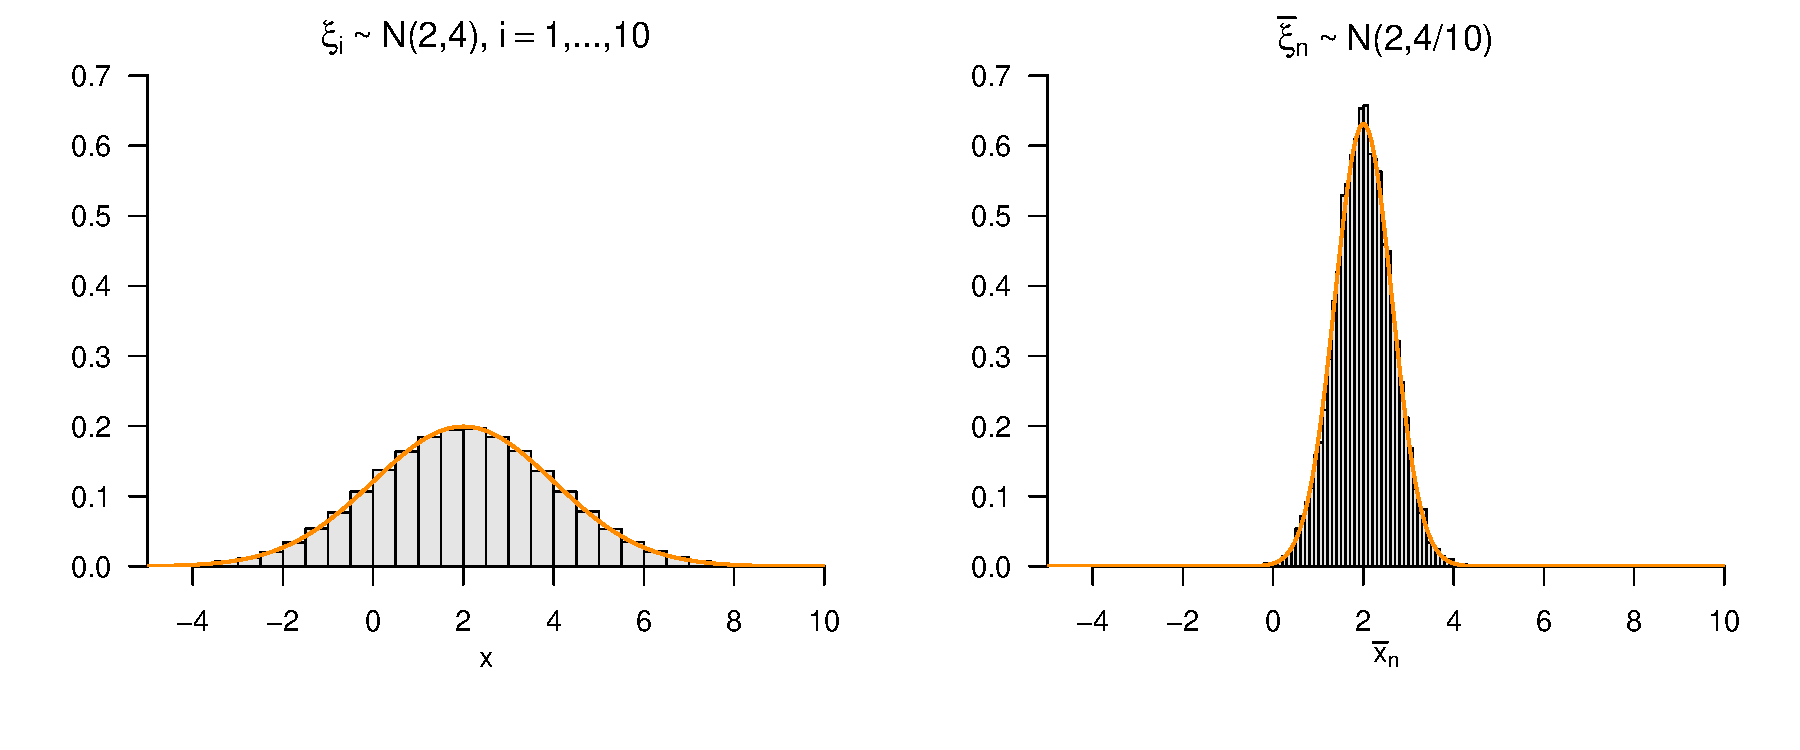
\includegraphics[width=1\linewidth]{8_Abbildungen/wtfi_8_mittelwert} \end{center}
\vfill
\end{frame}

\begin{frame}{Mittelwerttransformation}
\protect\hypertarget{mittelwerttransformation-2}{}
\vspace{2mm}
\footnotesize

\underline{Beweis} \setstretch{.9} \tiny

Wir halten zunächst fest, dass mit dem Theorem zur Summe von unabhängig
normalverteilten Zufallsvariablen gilt, dass
\(\bar{\xi}_n = \frac{1}{n}\ups\) mit
\(\ups := \sum_{i=1}^n \xi_i \sim N(n\mu,n\sigma^2)\). Einsetzen in das
univariate WDF Transformationstheorem für lineare Funktionen ergibt dann
\begin{align}
\begin{split}
p_{\bar{\xi}_n}(\bar{x}_n)
& = \frac{1}{|1/n|}N\left(n\bar{x}_n; n\mu , n\sigma^2 \right) \\
& = \frac{n}{\sqrt{2\pi n\sigma^2}}\exp\left(-\frac{1}{2n\sigma^2}
\left(n\bar{x}_n - n\mu\right)^2 \right) \\
& = \frac{n}{\sqrt{2\pi n\sigma^2}}\exp\left(-\frac{1}{2n\sigma^2}
\left(n\bar{x}_n - n\mu\right)^2 \right) \\
& = nn^{-\frac{1}{2}}\frac{1}{\sqrt{2\pi\sigma^2}}
\exp\left(
            -\frac{(n\bar{x}_n)^2}{2n\sigma^2}
            + \frac{2(n\bar{x}_n)(n\mu)}{2n\sigma^2}
            - \frac{(n\mu)^2}{2n\sigma^2}
         \right) \\
& = \sqrt{n}\frac{1}{\sqrt{2\pi\sigma^2}}
\exp\left(
            -\frac{n\bar{x}_n^2}{2\sigma^2}
            + \frac{2n\bar{x}_n\mu}{2\sigma^2}
            - \frac{n\mu^2}{2\sigma^2}
         \right) \\
& = \frac{1}{1/\sqrt{n}}\frac{1}{\sqrt{2\pi\sigma^2}}
\exp\left(
            -\frac{\bar{x}_n^2}{2(\sigma^2/n)}
            + \frac{2\bar{x}_n\mu}{2(\sigma^2/n)}
            - \frac{\mu^2}{2(\sigma^2/n)}
         \right) \\
& = \frac{1}{\sqrt{2\pi(\sigma^2/n)}}
\exp\left(-\frac{1}{2(\sigma^2/n)}
            (\bar{x}_n - \mu)^2
         \right) \\
& = N\left(\bar{x}_n;\mu,\sigma^2/n \right)
\end{split}
\end{align}
\end{frame}

\begin{frame}{}
\protect\hypertarget{section-8}{}
\setstretch{1.6}
\large

Vorbemerkungen

Transformationstheoreme

\textbf{Standardtransformationen}

\normalsize

\begin{itemize}
\tightlist
\item
  Summentransformation
\item
  Mittelwerttransformation
\item
  \textbf{\(Z\)-Transformation}
\item
  \(\chi^2\)-Transformation
\item
  \(T\)-Transformation
\item
  \(F\)-Transformation
\end{itemize}

\large

Selbstkontrollfragen
\end{frame}

\begin{frame}{\(Z\)-Transformation}
\protect\hypertarget{z-transformation}{}
\small
\begin{definition}[$z$-Zufallsvariable]
\justifying
$Z$ sei eine Zufallsvariable mit Ergebnisraum  $\mathbb{R}$ und WDF
\begin{equation}
p : \mathbb{R} \to \mathbb{R}_{>0}, z \mapsto p(z) := \frac{1}{\sqrt{2\pi}}\exp\left(-\frac{1}{2}z^2\right).
\end{equation}
Dann sagen wir, dass $Z$ einer \textit{$z$-Verteilung (oder Standardnormalverteilung)}
unterliegt und nennen $Z$ eine \textit{$z$-Zufallsvariable}. Wir kürzen dies mit
$Z \sim N(0,1)$ ab. Die WDF einer $z$-Zufallsvariable bezeichnen wir mit
\begin{equation}
N(z;0,1) := \frac{1}{\sqrt{2\pi}}\exp\left(-\frac{1}{2}z^2\right).
\end{equation}
\end{definition}

Bemerkung

\begin{itemize}
\tightlist
\item
  Eine \(z\)-Zufallsvariable ist eine normalverteilte Zufallsvariable
  mit \(\mu := 0\) und \(\sigma^2 := 1\).
\end{itemize}
\end{frame}

\begin{frame}{\(Z\)-Transformation}
\protect\hypertarget{z-transformation-1}{}
Wahrscheinlichkeitsdichtefunktion einer \(z\)-Zufallsvariable \vfill
\vspace{5mm}

\begin{center}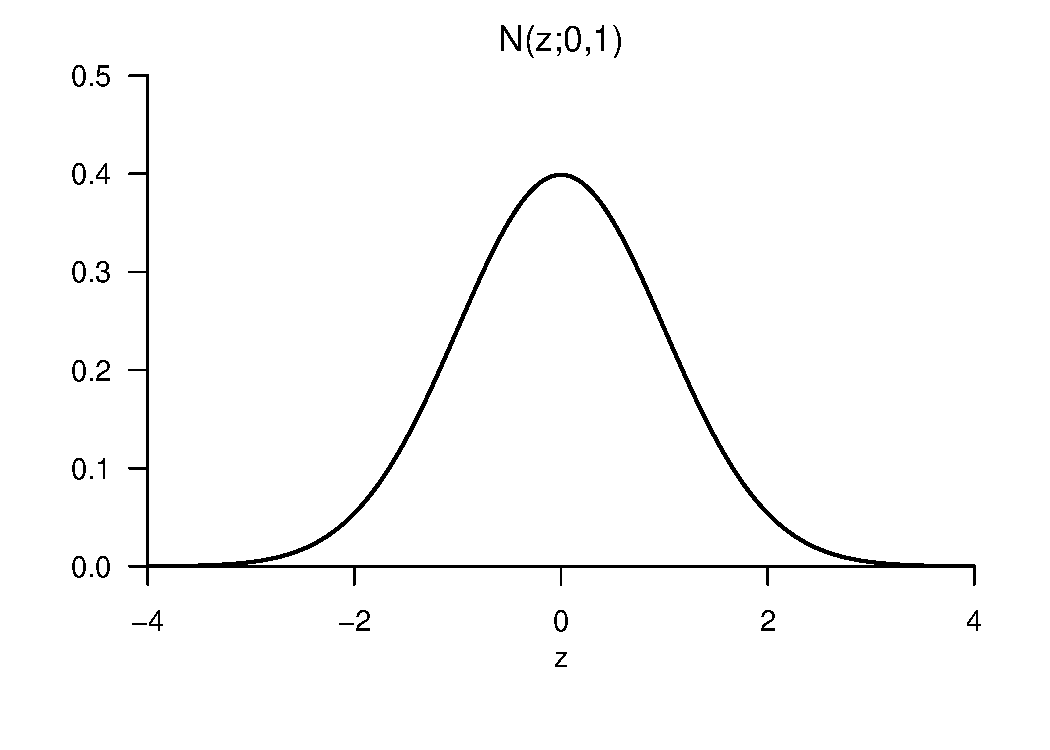
\includegraphics[width=0.7\linewidth]{8_Abbildungen/wtfi_8_z_verteilung} \end{center}
\vfill
\end{frame}

\begin{frame}{\(Z\)-Transformation}
\protect\hypertarget{z-transformation-2}{}
\small
\begin{theorem}[$Z$-Transformation]
\justifying
\normalfont
Es sei $y \sim N(\mu,\sigma^2)$ eine normalverteilte Zufallsvariable. Dann ist
die Zufallsvariable
\begin{equation}
Z := \frac{y - \mu}{\sigma}
\end{equation}
eine $Z$-verteilte Zufallsvariable, es gilt also $Z \sim N(0,1)$.
\end{theorem}

\footnotesize

Bemerkungen

\begin{itemize}
\item
  \justifying Wir benutzen hier den Bezeichner \(y\) für eine
  normalverteilte Zufallsvariable. Werte, die diese Zufallsvariable
  annehmen kann, bezeichnen wir in der Folge mit \(\tilde{y}\).
\item
  \justifying \(Z\) wird hier als \((y-\mu)/\sigma\) definiert. Dass ein
  solches \(Z\) aber eine \(z\)-Zufallsvariable ist, muss bewiesen
  werden und ergibt sich nicht einfach durch die Wahl des Bezeichners
  für \((y - \mu)/\sigma\), welcher hier zufällig auch \(Z\) lautet. In
  analoger Form gilt diese Bemerkung auch für alle weiteren betrachteten
  Transformationen.
\item
  Die \(Z\)-Konfidenzintervallstatistik und die \(Z\)-Teststatistik sind
  wichtige Anwendungsfälle.
\end{itemize}
\end{frame}

\begin{frame}{Z-Transformation}
\protect\hypertarget{z-transformation-3}{}
\vfill
\vspace{5mm}

\begin{center}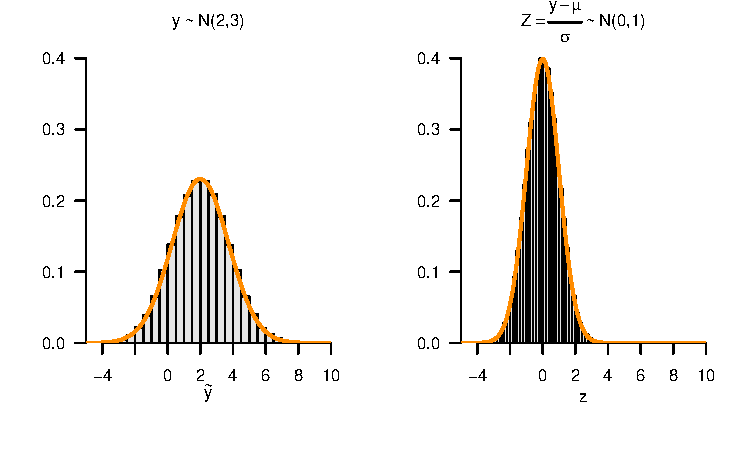
\includegraphics[width=1\linewidth]{8_Abbildungen/wtfi_8_z_transformation} \end{center}
\vfill
\end{frame}

\begin{frame}{\(Z\)-Transformation}
\protect\hypertarget{z-transformation-4}{}
\footnotesize

\underline{Beweis} \vspace{2mm}

Wir nutzen das univariate WDF Transformationstheorem für linear-affine
Funktionen. Dazu halten wir zunächst fest, dass die \(Z\)-Transformation
einer Funktion der Form \begin{equation}
\zeta : \mathbb{R} \to \mathbb{R}, \tilde{y} \mapsto \zeta(\tilde{y}) := \frac{\tilde{y} - \mu}{\sigma} =: z
\end{equation} entspricht. Wir stellen weiterhin fest, dass die
Umkehrfunktion von \(\zeta\) durch \begin{equation}
\zeta^{-1} : \mathbb{R} \to \mathbb{R}, z \mapsto \zeta^{-1}(z) := \sigma z + \mu
\end{equation} gegeben ist, da für alle \(z \in \mathbb{R}\) mit
\(z = \frac{\tilde{y} - \mu}{\sigma}\) gilt, dass \begin{equation}
\zeta^{-1}(z)
= \zeta^{-1}\left(\frac{\tilde{y} - \mu}{\sigma}\right)
= \frac{\sigma(\tilde{y} - \mu)}{\sigma} + \mu
= \tilde{y} - \mu + \mu
= \tilde{y}.
\end{equation} Schließlich stellen wir fest, dass für die Ableitung
\(\zeta'\) von \(\zeta\) gilt, dass \begin{equation}
\zeta'(\tilde{y})
= \frac{d}{d\tilde{y}}\left(\frac{\tilde{y} - \mu}{\sigma} \right)
= \frac{d}{d\tilde{y}}\left(\frac{\tilde{y}}{\sigma} -\frac{\mu}{\sigma} \right)
= \frac{1}{\sigma}.
\end{equation}
\end{frame}

\begin{frame}{\(Z\)-Transformation}
\protect\hypertarget{z-transformation-5}{}
\footnotesize

\underline{Beweis (fortgeführt)} \vspace{2mm}

Einsetzen in das univariate WDF Transformationstheorem für lineare
Funktionen ergibt dann \begin{align}
\begin{split}
p_\zeta(z)
& = \frac{1}{|1/\sigma|}N\left(\sigma z + \mu; \mu , \sigma^2 \right) \\
& = \frac{1}{1/\sqrt{\sigma^2}}\frac{1}{\sqrt{2\pi\sigma^2}}\exp\left(-\frac{1}{2\sigma^2}\left(\sigma z + \mu - \mu\right)^2 \right) \\
& = \frac{\sqrt{\sigma^2}}{\sqrt{2\pi\sigma^2}}\exp\left(-\frac{1}{2\sigma^2}\sigma^2 z^2\right)\\
& = \frac{1}{\sqrt{2\pi}}\exp\left(-\frac{1}{2} z^2\right)\\
& = N(z;0,1)
\end{split}
\end{align} also, dass \(Z \sim N(0,1)\). \(Z\) ist also eine
\(z\)-Zufallsvariable.
\end{frame}

\begin{frame}{}
\protect\hypertarget{section-9}{}
\setstretch{1.6}
\large

Vorbemerkungen

Transformationstheoreme

\textbf{Standardtransformationen}

\normalsize

\begin{itemize}
\tightlist
\item
  Summentransformation
\item
  Mittelwerttransformation
\item
  \(Z\)-Transformation
\item
  \textbf{\(\chi^2\)-Transformation}
\item
  \(T\)-Transformation
\item
  \(F\)-Transformation
\end{itemize}

\large

Selbstkontrollfragen
\end{frame}

\begin{frame}{\(\chi^2\)-Transformation}
\protect\hypertarget{chi2-transformation}{}
\small
\begin{definition}[$\chi^2$-Zufallsvariable]
\justifying
$U$ sei eine Zufallsvariable mit Ergebnisraum $\mathbb{R}_{>0}$ und WDF
\begin{equation}
p : \mathbb{R}_{>0} \to \mathbb{R}_{>0},
u \mapsto p(u)
:= \frac{1}{\Gamma\left(\frac{n}{2}\right)2^{\frac{n}{2}}}
u^{\frac{n}{2}-1}\exp\left(-\frac{1}{2}u\right),
\end{equation}
wobei $\Gamma$ die Gammafunktion bezeichne. Dann sagen wir, dass $U$ einer
$\chi^2$-Verteilung mit $n$ Freiheitsgraden unterliegt und nennen $U$ eine
$\chi^2$-Zufallsvariable mit $n$ Freiheitsgraden. Wir kürzen dies mit
$U \sim \chi^2(n)$ ab. Die WDF einer $\chi^2$-Zufallsvariable bezeichnen wir mit
\begin{equation}
\chi^2(u;n) :=
\frac{1}{\Gamma\left(\frac{n}{2}\right)2^{\frac{n}{2}}}
u^{\frac{n}{2}-1}\exp\left(-\frac{1}{2}u\right).
\end{equation}
\end{definition}

Bemerkung

\begin{itemize}
\tightlist
\item
  Die WDF der \(\chi^2\)-Verteilung entspricht der WDF
  \(G\left(u;\frac{n}{2},2\right)\) einer Gammaverteilung.
\end{itemize}
\end{frame}

\begin{frame}{\(\chi^2\)-Transformation}
\protect\hypertarget{chi2-transformation-1}{}
Wahrscheinlichkeitsdichtefunktionen von \(\xi^2\)-Zufallsvariablen

\vfill
\center

\begin{center}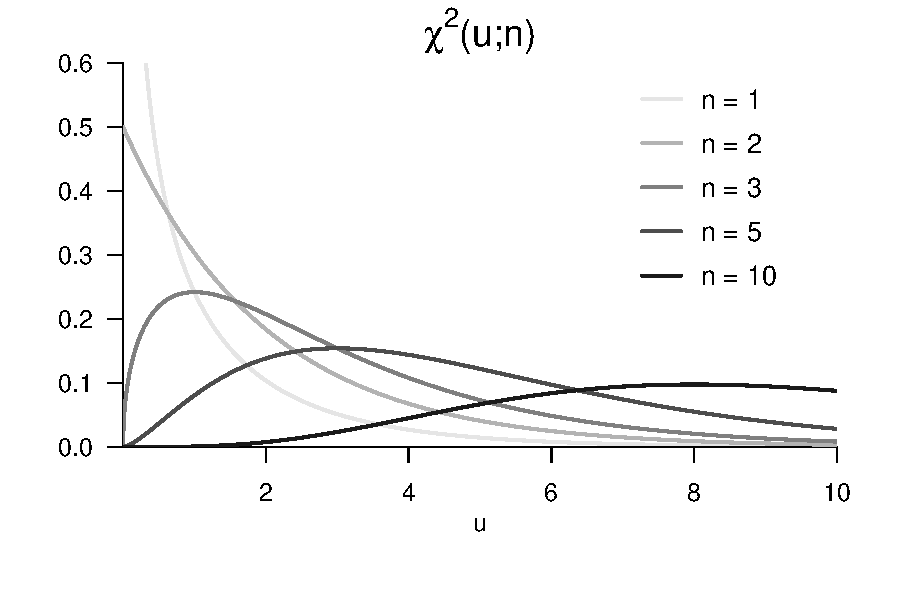
\includegraphics[width=0.8\linewidth]{8_Abbildungen/wtfi_8_chi2_wdf} \end{center}
\small

Steigendes \(n\) verbreitert \(\chi^2(u;n)\) und verschiebt Masse zur
größeren Werten.
\end{frame}

\begin{frame}{\(\chi^2\)-Transformation}
\protect\hypertarget{chi2-transformation-2}{}
\small
\begin{theorem}[$\chi^2$-Transformation]
\justifying
\normalfont
$Z_1,...,Z_n \sim N(0,1)$ seien unabhängig und identisch verteilte $z$-Zufallsvariablen.
Dann ist die Zufallsvariable
\begin{equation}
U := \sum_{i=1}^n Z_i^2
\end{equation}
eine $\chi^2$-verteilte Zufallsvariable mit $n$ Freiheitsgraden, es gilt also
$U \sim \chi^2(n)$. Insbesondere gilt für $Z \sim N(0,1)$ und $U := Z^2$, dass
$U \sim \chi^2(1)$.
\end{theorem}

\footnotesize

Bemerkungen

\begin{itemize}
\tightlist
\item
  Die \(U\)-Konfidenzintervallstatistik ist ein wichtiger
  Anwendungsfall.
\item
  \(t\)- und \(f\)-Zufallsvariablen sind wichtige Anwendungsfälle.
\end{itemize}
\end{frame}

\begin{frame}{\(\chi^2\)-Transformation}
\protect\hypertarget{chi2-transformation-3}{}
\vfill
\vspace{5mm}

\begin{center}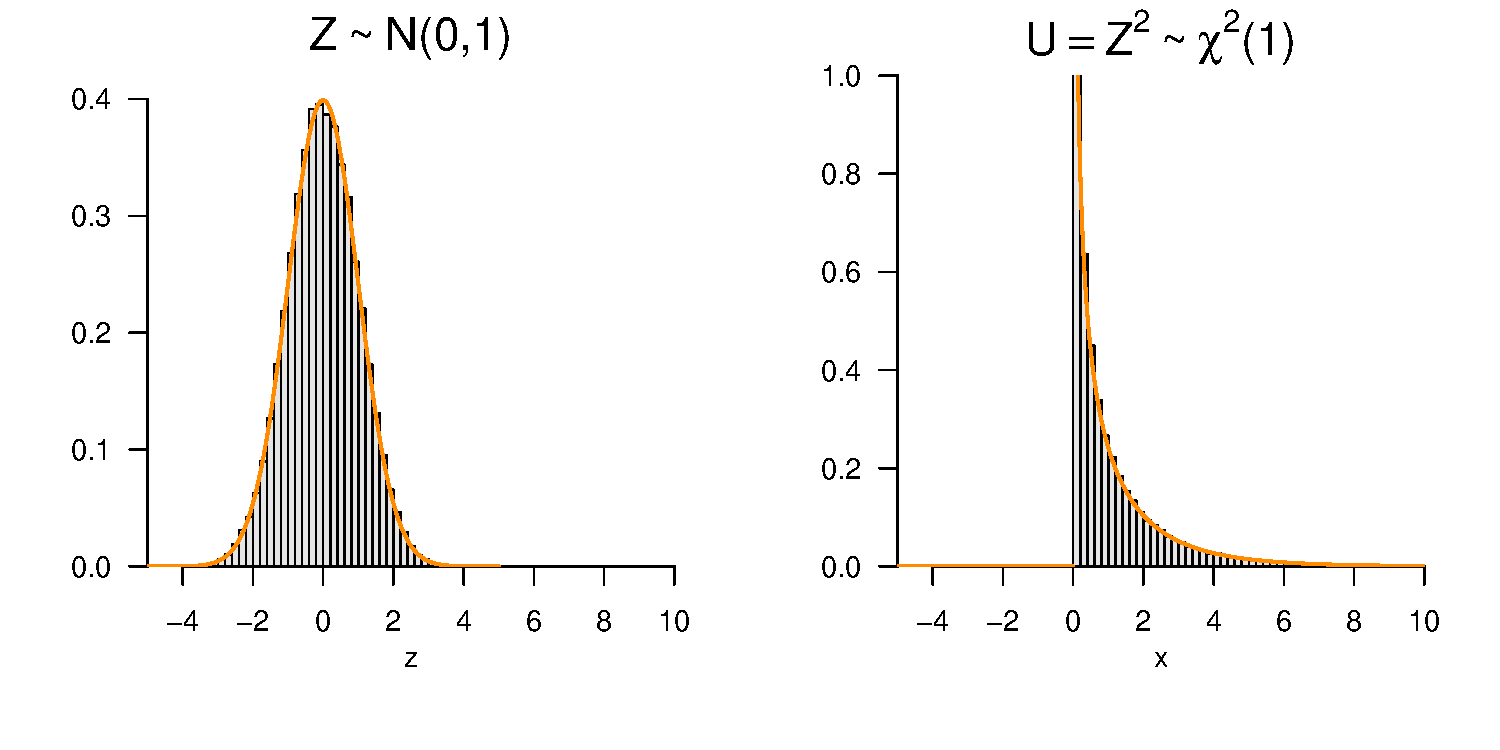
\includegraphics[width=0.9\linewidth]{8_Abbildungen/wtfi_8_chi2_transform} \end{center}
\vfill
\end{frame}

\begin{frame}{\(\chi^2\)-Transformation}
\protect\hypertarget{chi2-transformation-4}{}
\footnotesize

\underline{Beweis} \vspace{1mm}

Wir zeigen das Theorem nur für den Fall \(n := 1\) mithilfe des WDF
Transformationstheorems für stückweise bijektive Abbildungen. Danach ist
die WDF einer Zufallsvariable \(U := f(Z)\), welche aus der
Transformation einer Zufallsvariable \(Z\) mit WDF \(p_\zeta\) durch
eine stückweise bijektive Abbildung hervorgeht, gegeben durch
\begin{equation}\label{eq:piecewise_pdf_transform}
p_U(u) = \sum_{i=1}^k 1_{\mathcal{U}_i} \frac{1}{|f'_i(f_i^{-1}(u))|}p_\zeta\left(f_i^{-1} (u)\right).
\end{equation} Wir definieren \begin{equation}
\mathcal{U}_1 := ]-\infty,0[,
\mathcal{U}_2 := ]0,\infty[, \mbox{ und }
\mathcal{U}_i := \mathbb{R}_{>0} \mbox{ für } i = 1,2,
\end{equation} sowie \begin{equation}
f_i : \mathcal{Z}_i \to \mathcal{U}_i, x \mapsto f_i(z) := z^2 =: u \mbox{ für } i = 1,2.
\end{equation} Die Ableitung und die Umkehrfunktion der \(f_i\) ergeben
sich zu \begin{equation}
f_i' : \mathcal{Z}_i \to \mathcal{Z}_i, x \mapsto f_i'(z) = 2z \mbox{ für } i = 1,2,
\end{equation} und \begin{equation}
f_1^{-1} : \mathcal{U}_1 \to \mathcal{U}_1, u \mapsto f_1^{-1}(u) = - \sqrt{u}
\mbox{ und }
f_2^{-1} : \mathcal{U}_2 \to \mathcal{U}_2, u \mapsto f_2^{-1}(u) = \sqrt{u},
\end{equation} respektive.
\end{frame}

\begin{frame}{\(\chi^2\)-Transformation}
\protect\hypertarget{chi2-transformation-5}{}
\footnotesize

\underline{Beweis (fortgeführt)} \vspace{1mm}

Einsetzen in Gleichung \eqref{eq:piecewise_pdf_transform} ergibt dann
\begin{align}
\begin{split}
p_U(u)
& = 1_{\mathcal{U}_1}(u) \frac{1}{|f'_1(f_1^{-1}(u))|}p_\zeta\left(f_1^{-1} (u)\right)
  + 1_{\mathcal{U}_2}(u) \frac{1}{|f'_2(f_2^{-1}(u))|}p_\zeta\left(f_2^{-1} (u)\right) \\
& = \frac{1}{|2(-\sqrt{u})|}\frac{1}{\sqrt{2\pi}}\exp\left(-\frac{1}{2}(-\sqrt{u})^2\right)
  + \frac{1}{|2( \sqrt{u})|}\frac{1}{\sqrt{2\pi}}\exp\left(-\frac{1}{2}( \sqrt{u})^2\right) \\
& = \frac{1}{2\sqrt{u}}\frac{1}{\sqrt{2\pi}}\exp\left(-\frac{1}{2}u\right)
  + \frac{1}{2\sqrt{u}}\frac{1}{\sqrt{2\pi}}\exp\left(-\frac{1}{2}u\right)\\
& = \frac{1}{\sqrt{2\pi}}\frac{1}{\sqrt{u}}\exp\left(-\frac{1}{2}u\right).
\end{split}
\end{align} Andererseits gilt, dass mit
\(\Gamma\left(\frac{1}{2}\right) = \sqrt{\pi}\), die PDF einer
\(\chi^2\)-Zufallsvariable \(U\) mit \(n = 1\) durch \begin{equation}
\frac{1}{\Gamma\left(\frac{1}{2}\right)2^{\frac{1}{2}}} u^{\frac{1}{2}-1}\exp\left(-\frac{1}{2}u\right)
= \frac{1}{\sqrt{2\pi}}\frac{1}{\sqrt{u}}\exp\left(-\frac{1}{2}u\right)
\end{equation} gegeben ist. Also gilt, dass wenn \(Z \sim N(0,1)\) ist,
dann ist \(U := Z^2 \sim \chi^2(1)\).
\end{frame}

\begin{frame}{}
\protect\hypertarget{section-10}{}
\setstretch{1.6}
\large

Vorbemerkungen

Transformationstheoreme

\textbf{Standardtransformationen}

\normalsize

\begin{itemize}
\tightlist
\item
  Summentransformation
\item
  Mittelwerttransformation
\item
  \(Z\)-Transformation
\item
  \(\chi^2\)-Transformation
\item
  \textbf{\(T\)-Transformation}
\item
  \(F\)-Transformation
\end{itemize}

\large

Selbstkontrollfragen
\end{frame}

\begin{frame}{\(T\)-Transformation}
\protect\hypertarget{t-transformation}{}
\small
\begin{definition}[$t$-Zufallsvariable]
\justifying
$T$ sei eine Zufallsvariable mit Ergebnisraum $\mathbb{R}$ und WDF
\begin{equation}
p : \mathbb{R} \to \mathbb{R}_{>0}, t \mapsto p(t)
:= \frac{\Gamma\left(\frac{n+1}{2}\right)}{\sqrt{n\pi}\Gamma\left(\frac{n}{2}\right)}
\left(1 + \frac{t^2}{n} \right)^{-\frac{n+1}{2}},
\end{equation}
wobei $\Gamma$ die Gammafunktion bezeichne. Dann sagen wir, dass $T$ einer
$t$-Verteilung mit $n$ Freiheitsgraden unterliegt und nennen $T$ eine $t$-Zufallsvariable
mit $n$ Freiheitsgraden. Wir kürzen dies mit $T \sim t(n)$ ab. Die WDF einer
$t$-Zufallsvariable bezeichnen wir mit
\begin{equation}
T(t;n) := \frac{\Gamma\left(\frac{n+1}{2}\right)}{\sqrt{n\pi}\Gamma\left(\frac{n}{2}\right)}
\left(1 + \frac{t^2}{n} \right)^{-\frac{n+1}{2}}.
\end{equation}
\end{definition}
\end{frame}

\begin{frame}{\(T\)-Transformation}
\protect\hypertarget{t-transformation-1}{}
Wahrscheinlichkeitsdichtefunktionen von \(t\)-Zufallsvariablen
\vspace{5mm}

\begin{center}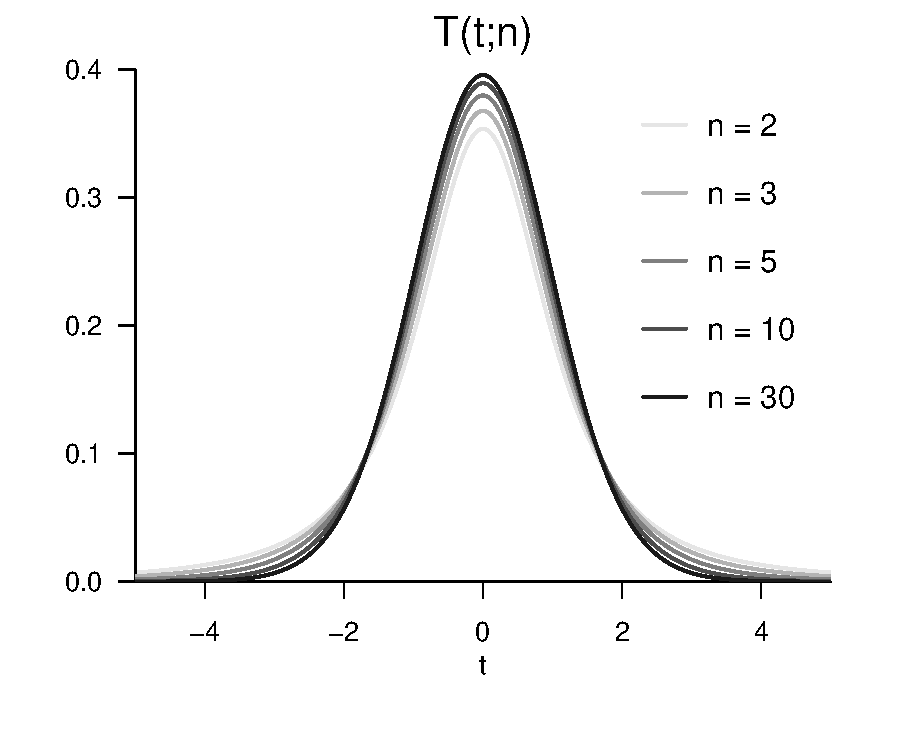
\includegraphics[width=0.6\linewidth]{8_Abbildungen/wtfi_8_t_wdf} \end{center}
\vspace{-3mm}
\footnotesize

\begin{itemize}
\tightlist
\item
  Die Verteilung ist um 0 symmetrisch
\item
  Steigendes \(n\) verschiebt Wahrscheinlichkeitsmasse aus den Ausläufen
  zum Zentrum.
\item
  Ab \(n = 30\) gilt \(T(t;n) \approx N(0,1)\).
\end{itemize}
\end{frame}

\begin{frame}{\(T\)-Transformation}
\protect\hypertarget{t-transformation-2}{}
\small
\begin{theorem}[$T$-Transformation]
\justifying
\normalfont
$Z \sim N(0,1)$ sei eine  $z$-Zufallsvariable, $U \sim \chi^2(n)$ sei eine
$\chi^2$-Zufallsvariable mit  $n$ Freiheitsgraden, und $Z$ und $U$ seien
unabhängige Zufallsvariablen. Dann ist die Zufallsvariable
\begin{equation}
T := \frac{Z}{\sqrt{U/n}}
\end{equation}
eine $t$-verteilte Zufallsvariable mit $n$ Freiheitsgraden, es gilt also $T \sim t(n)$.
\end{theorem}

\footnotesize

Bemerkungen

\begin{itemize}
\tightlist
\item
  Das Theorem geht auf Student (1908) zurück.
\item
  Das Theorem ist das zentrale Resultat der Frequentistischen Statistik.
\item
  Zabell (2008) gibt hierzu einen historischen Überblick.
\item
  Die \(T\)-Konfidenzintervallstatistik und die \(T\)-Teststatistik sind
  wichtige Anwendungsfälle.
\end{itemize}
\end{frame}

\begin{frame}{\(T\)-Transformation}
\protect\hypertarget{t-transformation-3}{}
\vfill
\vspace{3mm}

\begin{center}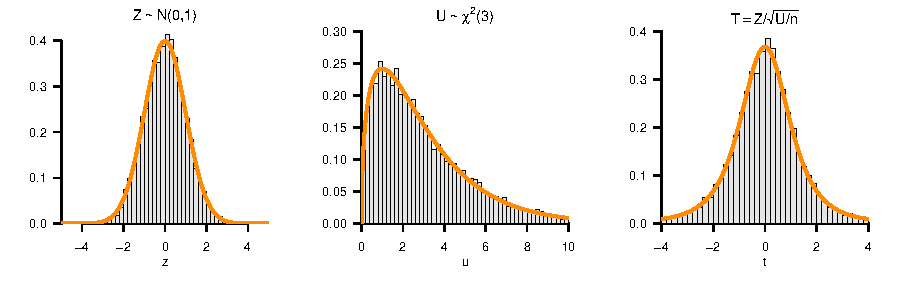
\includegraphics[width=1\linewidth]{8_Abbildungen/wtfi_8_t_transform} \end{center}
\vfill
\end{frame}

\begin{frame}{\(T\)-Transformation}
\protect\hypertarget{t-transformation-4}{}
\footnotesize

\underline{Beweis} \vspace{1mm}

Wir halten zunächst fest, dass die zweidimensionale WDF der gemeinsamen
(unabhängigen) Verteilung von \(Z\) und \(U\) durch \begin{equation}
p_{Z,U}(z,u)
=
\frac{1}{\sqrt{2\pi}}\exp\left(-\frac{1}{2}z^2\right)
\frac{1}{\Gamma(\frac{n}{2})2^{\frac{n}{2}}}u^{\frac{n}{2}-1} \exp\left(-\frac{1}{2}u\right).
\end{equation} gegeben ist. Wir betrachten dann die multivariate
vektorwertige Abbildung \begin{equation}
f : \mathbb{R}^2 \to \mathbb{R}^2,
(z,u)
\mapsto
f(z,u)
:=
\left(\frac{z}{\sqrt{u/n}},u\right)
=:
(t,w)
\end{equation} und benutzen das multivariate WDF Transformationstheorem
für bijektive Abbildungen um die WDF von \((t,w)\) herzuleiten. Dazu
erinnern wir uns, dass wenn \(\xi\) ein \(n\)-dimensionaler
Zufallsvektor mit WDF \(p_\xi\) und \(\ups := f(\xi)\) für eine
differenzierbare und bijektive Abbildung
\(f : \mathbb{R}^n \to \mathbb{R}^n\) ist, die WDF des Zufallsvektors
\(\ups\) durch \begin{equation}\label{eq:pdftmv}
p_\ups : \mathbb{R}^n \to \mathbb{R}_{\ge 0},
y \mapsto p_\ups(y) :=
\frac{1}{|J^f\left(f^{-1}(y)\right)|}p_\xi\left(f^{-1}(y)\right)
\end{equation} gegeben ist. Für die im vorliegenden Fall betrachtete
Abbildung halten wir zunächst fest, dass \begin{equation}
f^{-1}:\mathbb{R}^2 \to \mathbb{R}^2,
(t,w)
\mapsto
f^{-1}
(t,w)
:=\left(\sqrt{w/n}t, w\right).
\end{equation}
\end{frame}

\begin{frame}{\(T\)-Transformation}
\protect\hypertarget{t-transformation-5}{}
\footnotesize

\underline{Beweis (fortgeführt)} \vspace{1mm}

Dies ergibt sich direkt aus \begin{equation}
f^{-1}(f(z,u))
=
f^{-1}\left(\frac{z}{\sqrt{u/n}},u\right)
=
\left(\frac{\sqrt{u/n}z}{\sqrt{u/n}}, u \right)
=
(z,u)
\mbox{ für alle }
(z,u)
\in \mathbb{R}^2.
\end{equation} Wir halten dann fest, dass die Determinante der
Jacobi-Matrix von \(f\) an der Stelle \((z,u)\) durch \begin{equation}
|J^f(z,u)|
=
\begin{vmatrix}
  \frac{\partial}{\partial z} \left(\frac{z}{\sqrt{u/n}}\right)
& \frac{\partial}{\partial u} \left(\frac{z}{\sqrt{u/n}}\right) \\
  \frac{\partial}{\partial z} u
& \frac{\partial}{\partial u} u\\
\end{vmatrix}
= \left(\frac{v}{n}\right)^{-1/2},
\end{equation} gegeben ist, sodass folgt, dass \begin{equation}
\frac{1}{|J^f\left(f^{-1}(z,u)\right)|}
= \left(\frac{w}{n}\right)^{1/2}.
\end{equation} Einsetzen in Gleichung \eqref{eq:pdftmv} ergibt dann
\begin{equation}
p_{T,W}(t,w) = \left(\frac{w}{n}\right)^{1/2}p_{Z,V}\left(\sqrt{w/n}t,w\right),
\end{equation}
\end{frame}

\begin{frame}{\(T\)-Transformation}
\protect\hypertarget{t-transformation-6}{}
\footnotesize

\underline{Beweis (fortgeführt)} \vspace{1mm}

Es folgt also \tiny \begin{align}
\begin{split}
p_T(t)
& =
\int_0^\infty  p_{T,W}(t,w)
\,dw                                                    \\
& =
\int_0^\infty
\left(\frac{w}{n}\right)^{1/2}
p_{Z,V}\left(\sqrt{w/n}t,w\right)
\,dw  \\
& =
\int_0^\infty
\frac{1}{\sqrt{2\pi}}\exp\left(-\frac{1}{2}(\sqrt{w/n}t)^2\right)
\frac{1}{\Gamma(\frac{n}{2})2^{\frac{n}{2}}}w^{\frac{n}{2}-1} \exp\left(-\frac{1}{2}w\right)
\left(\frac{w}{n}\right)^{1/2}
\,dw \\
& =
\frac{1}{\sqrt{2\pi}}\frac{1}{\Gamma(\frac{n}{2})2^{\frac{n}{2}}n^{\frac{1}{2}}}
\int_0^\infty
\exp\left(-\frac{1}{2}\frac{w}{n}t^2\right)
w^{\frac{n}{2}-1} \exp\left(-\frac{1}{2}w\right)w^{1/2}
\,dw \\
& =
\frac{1}{\sqrt{2\pi}}\frac{1}{\Gamma(\frac{n}{2})2^{\frac{n}{2}}n^{\frac{1}{2}}}
\int_0^\infty
\exp\left(-\frac{1}{2}\frac{w}{n}t^2 -\frac{1}{2}w\right)
w^{\frac{n}{2}-1} w^{\frac{1}{2}}
\,dw \\
& =
\frac{1}{\sqrt{2\pi}}\frac{1}{\Gamma(\frac{n}{2})2^{\frac{n}{2}}n^{\frac{1}{2}}}
\int_0^\infty
\exp\left(-\frac{1}{2}\left(\frac{w}{n}t^2 + w\right)\right)
w^{\frac{n + 1}{2}-1}
\,dw \\
& =
\frac{1}{\sqrt{2\pi}}\frac{1}{\Gamma(\frac{n}{2})2^{\frac{n}{2}}n^{\frac{1}{2}}}
\int_0^\infty
\exp\left(-\frac{1}{2}\left(1 + \frac{t^2}{n}\right)\right)
w^{\frac{n + 1}{2}-1}
\,dw \\
\end{split}
\end{align}
\end{frame}

\begin{frame}{\(T\)-Transformation}
\protect\hypertarget{t-transformation-7}{}
\footnotesize

\underline{Beweis (fortgeführt)} \vspace{1mm}

Wir stellen dann fest, dass der Integrand auf der linken Seite der
obigen Gleichung dem Kern einer Gamma WDF mit Parametern
\(\alpha = \frac{n+1}{2}\) und \(\beta = \frac{2}{1+\frac{t^2}{n}}\)
entspricht, wie man leicht einsieht: \begin{align*}
\Gamma(w;\alpha,\beta)
= \frac{1}{\Gamma(\alpha)\beta^{\alpha}}w^{\alpha-1}\exp\left(-\frac{w}{\beta}\right) & \\
\Rightarrow
\Gamma\left(w;\frac{n+1}{2},\frac{2}{1+\frac{t^2}{n}}\right)
& = \frac{1}{\Gamma(\frac{n+1}{2})\left(\frac{2}{1+\frac{t^2}{n}}\right)^{\frac{n+1}{2}}}
w^{\frac{n+1}{2}-1}\exp\left(-\frac{w}{\frac{2}{1+\frac{t^2}{n}}}\right) \\
& = \frac{1}{\Gamma( \frac{n+1}{2})\left(\frac{2}{1+\frac{t^2}{n}}\right)^{ \frac{n+1}{2}}}
\exp\left(-\frac{1}{2}\left(1 + \frac{t^2}{n}\right)\right) w^{\frac{n+1}{2}-1}.
\end{align*}
\end{frame}

\begin{frame}{\(T\)-Transformation}
\protect\hypertarget{t-transformation-8}{}
\footnotesize

\underline{Beweis (fortgeführt)} \vspace{1mm}

Es ergibt sich also \begin{equation}
p_T(t)
=
\frac{1}{\sqrt{2\pi}}\frac{1}{\Gamma(\frac{n}{2})2^{\frac{n}{2}}n^{\frac{1}{2}}}
\int_0^\infty
\Gamma\left(w;\frac{n+1}{2},\frac{2}{1+\frac{t^2}{n}}\right)
\,dw .
\end{equation} Schließlich stellen wir fest, dass der Integralterm in
obiger Gleichung dem Normalisierungsterm einer Gamma WDF entspricht.
Abschließend ergibt sich also \begin{equation}
p_T(t) =
\frac{1}{\sqrt{2\pi}}\frac{1}{\Gamma(\frac{n}{2})2^{\frac{n}{2}}n^{\frac{1}{2}}}
\Gamma\left(\frac{n+1}{2}\right)\left(\frac{2}{1 + \frac{t^2}{n}} \right)^{\frac{n+1}{2}}.
\end{equation} Die Verteilung von \(Z/\sqrt{U/n}\) hat also die WDF
einer \(T\)-Zufallsvariable.

\(\hfill \Box\)
\end{frame}

\begin{frame}{}
\protect\hypertarget{section-11}{}
\setstretch{1.6}
\large

Vorbemerkungen

Transformationstheoreme

\textbf{Standardtransformationen}

\normalsize

\begin{itemize}
\tightlist
\item
  Summentransformation
\item
  Mittelwerttransformation
\item
  \(Z\)-Transformation
\item
  \(\chi^2\)-Transformation
\item
  \(T\)-Transformation
\item
  \textbf{\(F\)-Transformation}
\end{itemize}

\large

Selbstkontrollfragen
\end{frame}

\begin{frame}{\(F\)-Transformation}
\protect\hypertarget{f-transformation}{}
\small
\begin{definition}[$f$-Zufallsvariable]
\justifying
$F$ sei eine Zufallsvariable mit Ergebnisraum $\mathbb{R}_{>0}$ und WDF
\begin{equation}
p_F : \mathbb{R} \to \mathbb{R}_{>0}, f \mapsto p_F(f)
:= m^{\frac{m}{2}}n^{\frac{n}{2}}
   \frac{\Gamma\left(\frac{m+n}{2}\right)}{\Gamma\left(\frac{m}{2}\right)\Gamma\left(\frac{n}{2}\right)}
   \frac{f^{\frac{m}{2}-1}}{\left(1 + \frac{m}{n}f \right)^{\frac{m+n}{2}}},
\end{equation}
wobei $\Gamma$ die Gammafunktion bezeichne. Dann sagen wir, dass $F$ einer
$f$-Verteilung mit $n,m$ Freiheitsgraden unterliegt und nennen $F$ eine
$f$-Zufallsvariable mit $n,m$ Freiheitsgraden. Wir kürzen dies mit $F \sim f(n,m)$ ab.
Die WDF einer $f$-Zufallsvariable bezeichnen wir mit
\begin{equation}
F(f;n,m)
:= m^{\frac{m}{2}}n^{\frac{n}{2}}
   \frac{\Gamma\left(\frac{m+n}{2}\right)}{\Gamma\left(\frac{m}{2}\right)\Gamma\left(\frac{n}{2}\right)}
   \frac{f^{\frac{m}{2}-1}}{\left(1 + \frac{m}{n}f \right)^{\frac{m+n}{2}}}.
\end{equation}
\end{definition}
\end{frame}

\begin{frame}{\(F\)-Transformation}
\protect\hypertarget{f-transformation-1}{}
Wahrscheinlichkeitsdichtefunktionen von \(f\)-Zufallsvariablen
\vspace{5mm} \center

\begin{center}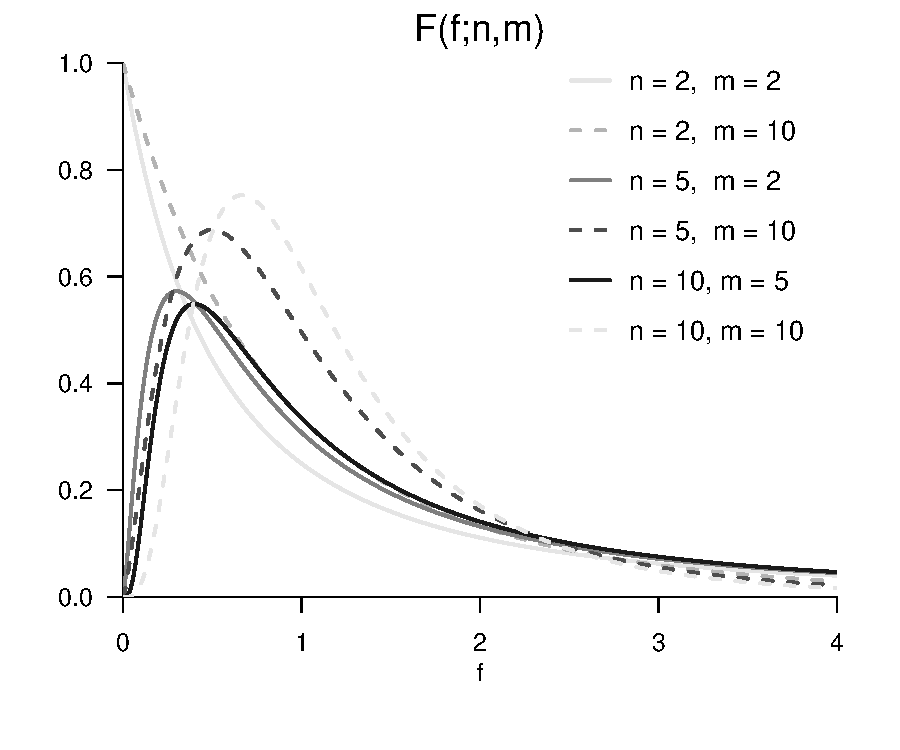
\includegraphics[width=0.7\linewidth]{8_Abbildungen/wtfi_8_f_wdf} \end{center}
\vfill
\end{frame}

\begin{frame}{\(F\)-Transformation}
\protect\hypertarget{f-transformation-2}{}
\small
\begin{theorem}[$F$-Transformation]
\justifying
\normalfont
$V \sim \chi^2(n)$ und $W \sim \chi^2(m)$ seien zwei unabhängige
$\chi^2$-Zufallfsvariablen mit $n$ und $m$ Freiheitsgraden, respektive.
Dann ist die Zufallsvariable
\begin{equation}
F := \frac{V/n}{W/m}
\end{equation}
eine $f$-verteilte Zufallsvariable mit $n,m$ Freiheitsgraden, es gilt also $F \sim f(n,m)$.
\end{theorem}

\footnotesize

Bemerkungen

\begin{itemize}
\tightlist
\item
  Wir verzichten auf einen Beweis
\item
  Das Theorem kann bewiesen werden, in dem man zunächst ein
  Transformationstheorem für Quotienten von Zufallsvariablen mithilfe
  des multivariaten Transformationstheorems und Marginalisierung
  herleitet und dieses Theorem dann auf die WDF von
  \(\chi^2\)-verteilten ZVen anwendet. Dabei ist die Regel zur
  Integration durch Substitution von zentraler Bedeutung.
\end{itemize}
\end{frame}

\begin{frame}{\(F\)-Transformation}
\protect\hypertarget{f-transformation-3}{}
\vspace{5mm}
\vfill

\begin{center}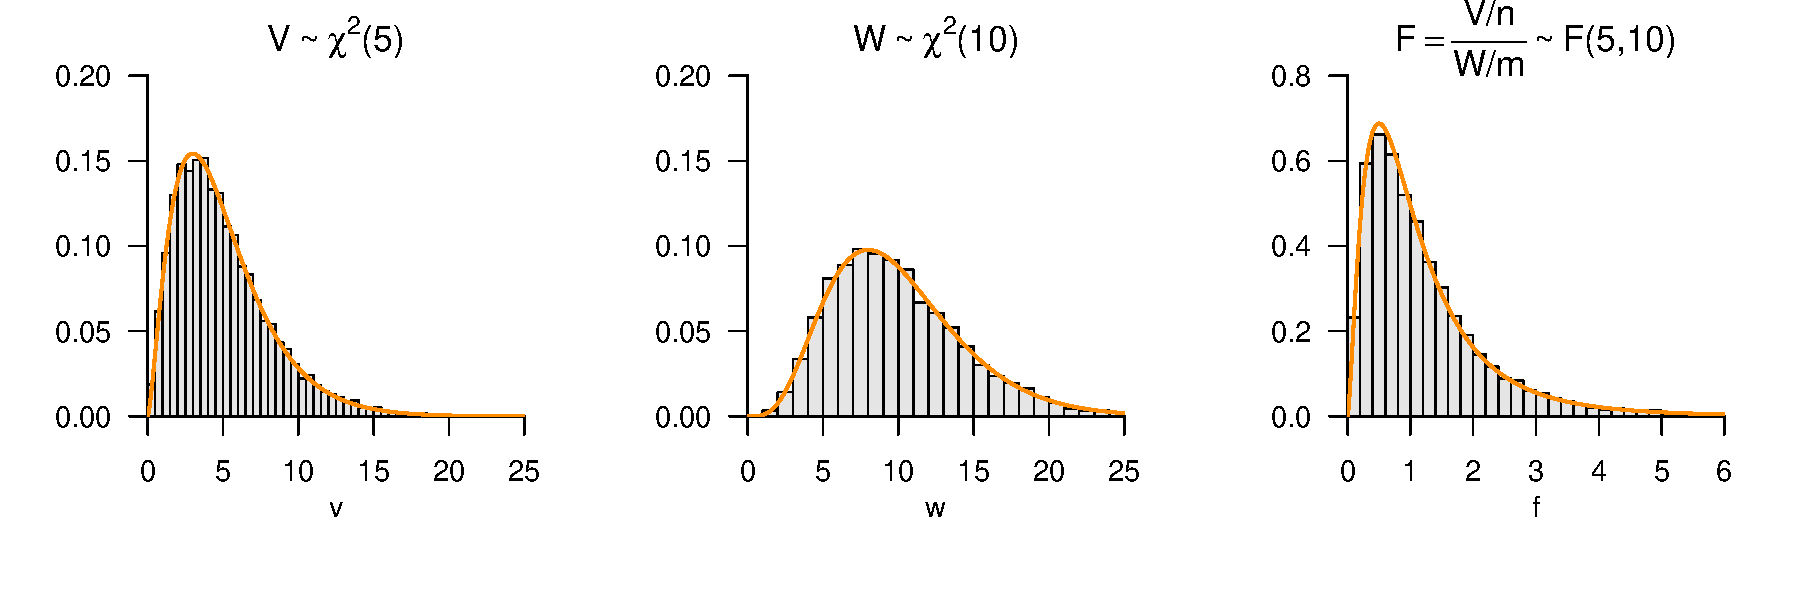
\includegraphics[width=1\linewidth]{8_Abbildungen/wtfi_8_f_transform} \end{center}
\vfill
\end{frame}

\begin{frame}{}
\protect\hypertarget{section-12}{}
\setstretch{1.6}
\large

Vorbemerkungen

Transformationstheoreme

Standardtransformationen

\normalsize

\begin{itemize}
\tightlist
\item
  Summentransformation
\item
  Mittelwerttransformation
\item
  \(Z\)-Transformation
\item
  \(\chi^2\)-Transformation
\item
  \(T\)-Transformation
\item
  \(F\)-Transformation
\end{itemize}

\textbf{Selbstkontrollfragen}
\end{frame}

\begin{frame}{Selbstkontrollfragen}
\protect\hypertarget{selbstkontrollfragen}{}
\small
\setstretch{1.5}
\begin{enumerate}
\item Erläutern Sie den Begriff der Transformation einer Zufallsvariable.
\item Erläutern Sie die zentrale Idee der Transformationstheoreme.
\item Erläutern Sie die Bedeutung der Standardtransformationen für die Statistik.
\item Geben Sie das Summentransformationstheorem wieder.
\item Geben Sie das Mittelwerttransformationstheorem wieder.
\item Geben Sie das $Z$-Transformationstheorem wieder.
\item Geben Sie das $\chi^2$-Transformationstheorem wieder.
\item Beschreiben Sie die WDF der $t$-Verteilung in Abhängigkeit ihrer Freiheitsgrade.
\item Geben Sie das $T$-Transformationstheorem wieder.
\item Geben Sie das $F$-Transformationstheorem wieder.
\end{enumerate}
\end{frame}

\begin{frame}{References}
\protect\hypertarget{references}{}
\footnotesize

\hypertarget{refs}{}
\begin{CSLReferences}{1}{0}
\leavevmode\vadjust pre{\hypertarget{ref-student_1908}{}}%
Student. 1908. {``The {Probable Error} of a {Mean}.''} \emph{Biometrika}
6 (1): 1--25.

\leavevmode\vadjust pre{\hypertarget{ref-zabell_2008}{}}%
Zabell, S. L. 2008. {``On {Student}'s 1908 {Article} {`{The Probable
Error} of a {Mean}'}.''} \emph{Journal of the American Statistical
Association} 103 (481): 1--7.
\url{https://doi.org/10.1198/016214508000000030}.

\end{CSLReferences}
\end{frame}

\end{document}
